
\newpage

\begin{flushright}
  \vspace{10cm}
  \rule{18cm}{5pt}
  \rule{18cm}{2pt}\vskip1cm
  \begin{center}
    \begin{bfseries}
      \Huge{\textbf{Building a Chatbot: Using AWS Lex}}\\
    \end{bfseries}
  \end{center}
  \vspace{1cm}
  \rule{18cm}{2pt}
  \rule{18cm}{5pt}
\end{flushright}
\newpage

\chapter{Bot RideRequest}
\section{Actions taken to perform the bot creation operation}
To create the "\textbf{TaxiRequest}" and "\textbf{SelfDriveRequest}" intents in AWS Lex, log in to your AWS account and access the AWS Management Console. From there, open the Amazon Lex service and either create a new bot. Once inside the bot, navigate to the "\textbf{Intents}" section and click on "\textbf{Create Intent}." For the "TaxiRequest" intent, name it accordingly and add sample utterances that users might say when requesting a taxi ride. Create the necessary slots to collect information like \textbf{pickup address,} \textbf{pickup date}, \textbf{pickup time}, and \textbf{vehicle type}. Configure prompts for each slot to prompt the user for the required details. Similarly, for the "SelfDriveRequest" intent, name it accordingly and add sample utterances related to self-drive requests. Create slots to collect information such as \textbf{arrival time}, \textbf{vehicle type}, and \textbf{number of vehicles}. Configure prompts for each slot to obtain the necessary details from the user. Define c\textbf{onfirmation prompts} for both intents using placeholders for variable values to confirm the user's request. Set up the \textbf{fulfillment logic} for each intent, including appropriate success and failure messages. Save the intent configurations and \textbf{build the bot} to apply the changes. These steps allow us to create the "TaxiRequest" and "SelfDriveRequest" intents in AWS Lex and we can customize them according to our requirements. Finally, \textbf{test the bot}, to check if it satisfies all the requirements. 


\section{Intents}
\subsection{TaxiRequest}
The "TaxiRequest" intent allows users to request a taxi ride. It collects information such as the customer's address for pickup, pickup date, and pickup time.
\subsubsection{Sample utterances: }
Can you call me a taxi? \newline
I need a taxi to the airport.\newline
I need a ride to the train station.\newline
I'm looking for a taxi service.\newline

\subsubsection{Create Custom Slot type Vehicle}
\begin{enumerate}
    \item Create a new, Custom slot type in the bot
    \item Slot name: Vehicle
    \item Slot type values(restrict to these values only) : 
    \begin{enumerate}
        \item Key = suv ; Values = SUV, suv, Suv
        \item Key = minivan ; Values =  Minivan, MiniVan, minivan
    \end{enumerate}
\end{enumerate}

\subsubsection{Slots \& Prompts }

\begin{table}[h]
\centering
\begin{tabular}{|>{\bfseries}m{4cm}|m{8cm}|m{5cm}|}
\hline
\textbf{Slots} & \textbf{Prompts} & \textbf{Slot Type} \\
\hline
\textbf{CustomerAddress} & Sure, you've selected a taxi ride. Could you please provide your address for pickup? & AMAZON.FreeFormInput \\
\hline
\textbf{PickupDate} & Thank you! When do you need the taxi? Please provide the pickup date. & AMAZON.Date \\
\hline
\textbf{PickupTime} & Great! What time would you like the taxi to arrive? Please provide the pickup time. & AMAZON.Time \\
\hline
\textbf{VehicleType} & What do you want today (SUV, Sedan, Minivan)? & AMAZON.Vehicle(custom built) \\
\hline
\textbf{NumberOfVehicles} & How many? & AMAZON.Number \\
\hline
\end{tabular}
\end{table}

\newpage
\subsubsection{Confirmation prompt:}
Use this prompt with placeholders for variable values (indicated using \{\} ), to get confirmation from the user(YES/NO).


\definecolor{backcolour}{RGB}{242, 242, 242}
\definecolor{bracketcolour}{RGB}{255, 0, 0}

\lstdefinelanguage{customlang}{
    moredelim=[s][\color{bracketcolour}]{\{}{\}},
    sensitive=false,
}

\lstset{
    backgroundcolor=\color{backcolour},
    basicstyle=\small\ttfamily,
    breaklines=true,
    captionpos=b,
    frame=single,
    keywordstyle=\color{blue},
    language=customlang, % Specify the custom language style
    numbers=left,
    numbersep=5pt,
    numberstyle=\tiny\color{gray},
    showspaces=false,
    showstringspaces=false,
    showtabs=false,
    stringstyle=\color{red},
    tabsize=2
}

\begin{lstlisting}[caption={Code snippet}]
You have requested for {NumberOfVehicles} {VehicleType} for pickup address 
{CustomerAddress}. Your pickup date is {PickupDate}, and your pickup time is {PickupTime}. Please confirm.
\end{lstlisting}

\subsubsection{Fulfillment :}
% \textbf{On success:} Your request has been placed successfully.
% \newline
% \textbf{In case of failure:} Oops!! Sorry, your request could not be placed at this moment. Please try again later.

\begin{table}[h]
\centering
\begin{tabular}{|m{4cm}|m{7cm}|}
\hline
\textbf{On success} & Your request has been placed successfully. \\
\hline
\textbf{In case of failure} & Oops!! Sorry, your request could not be placed at this moment. Please try again later. \\
\hline
\end{tabular}
\end{table}

% ----------------------------------------------------

\subsection{SelfDriveRequest}
The SelfDriveRequest intent is used to request a self-drive ride or car rental. It collects information about the vehicle type, number of vehicles, and pickup time.

\subsubsection{Sample utterances: }
I want to request a self-drive ride. \newline
I'm looking to rent a car for the day.\newline
I need a car to pick up my kids from school.\newline
I'm going to the airport and need a car to get there.\newline

\newpage
\subsubsection{Slots \& Prompts }
% \newpage
\begin{table}[h]
\centering
\begin{tabular}{|>{\bfseries}m{4cm}|m{8cm}|m{5cm}|}
\hline
\textbf{Slots} & \textbf{Prompts} & \textbf{Slot Type} \\
\hline
ArrivalTime & Sure, you've selected a self-drive ride. When are you coming TODAY to get your vehicle? & AMAZON.Time \\
\hline
VehicleType & What do you want today (SUV, Sedan, Minivan)? & AMAZON.Vehicle(custom built) \\
\hline
NumberOfVehicles & How many? & AMAZON.Number \\
\hline
\end{tabular}
\end{table}


% \newpage
\subsubsection{Confirmation prompt:}
Use this prompt with placeholders for variable values (indicated using \{\} ), to get confirmation from the user (YES/NO).


\definecolor{backcolour}{RGB}{242, 242, 242}
\definecolor{bracketcolour}{RGB}{255, 0, 0}

\lstdefinelanguage{customlang}{
    moredelim=[s][\color{bracketcolour}]{\{}{\}},
    sensitive=false,
}

\lstset{
    backgroundcolor=\color{backcolour},
    basicstyle=\small\ttfamily,
    breaklines=true,
    captionpos=b,
    frame=single,
    keywordstyle=\color{blue},
    language=customlang, % Specify the custom language style
    numbers=left,
    numbersep=5pt,
    numberstyle=\tiny\color{gray},
    showspaces=false,
    showstringspaces=false,
    showtabs=false,
    stringstyle=\color{red},
    tabsize=2
}

\begin{lstlisting}[caption={Code snippet}]
You have requested for {NumberOfVehicles} {VehicleType}, and you will be arriving at {ArrivalTime}. Please confirm.
\end{lstlisting}

\subsubsection{Fulfillment :}
% \textbf{On success:} Your request has been placed successfully.
% \newline
% \textbf{In case of failure:} Oops!! Sorry, your request could not be placed at this moment. Please try again later.

\begin{table}[h]
\centering
\begin{tabular}{|m{4cm}|m{7cm}|}
\hline
\textbf{On success} & Your request has been placed successfully. \\
\hline
\textbf{In case of failure} & Oops!! Sorry, your request could not be placed at this moment. Please try again later. \\
\hline
\end{tabular}
\end{table}
\newpage
\section{Screenshots}
\begin{figure}[htp]
    \centering
    \fbox{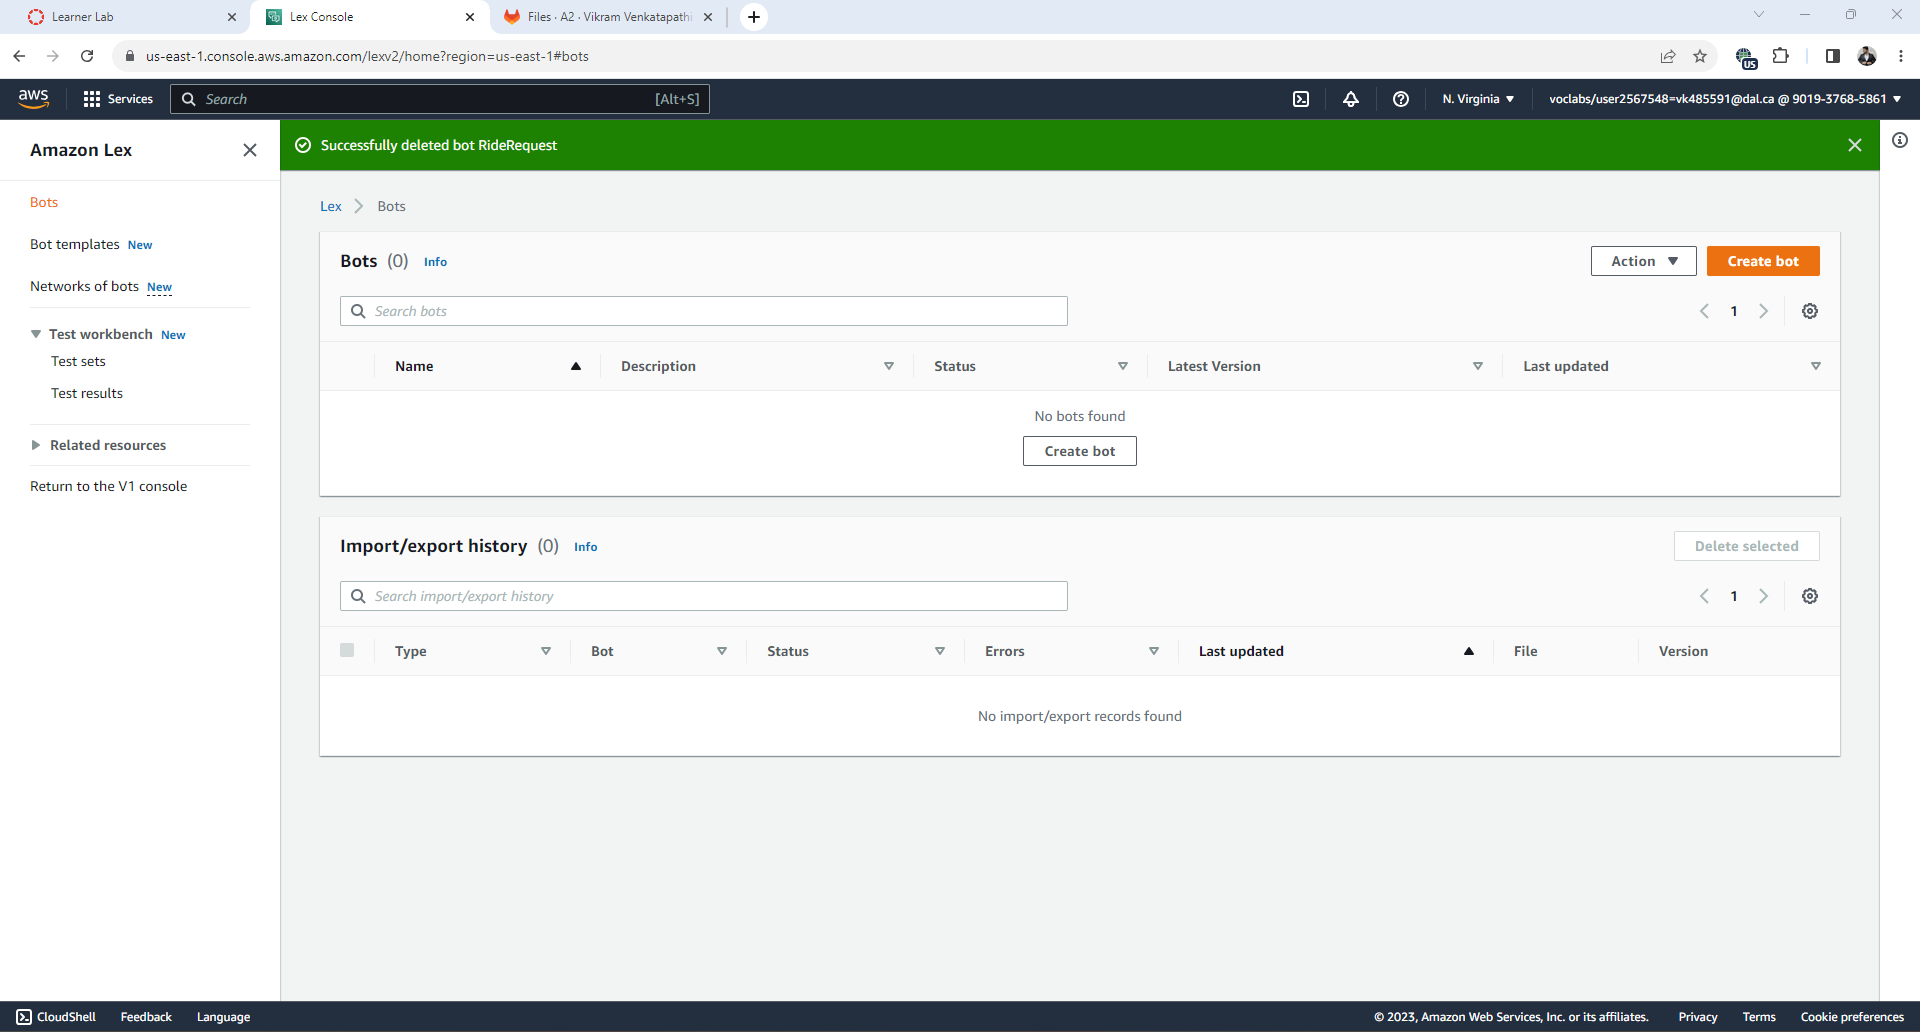
\includegraphics[scale=1, width=15cm,height=7.5cm]{PROBLEM 2/Screenshots/3. Lex/0. Empty bots.png}}
    \caption{\textbf{\textit{Empty bots section}}}
    \label{fig:}
\end{figure}
\begin{figure}[htp]
    \centering
    \fbox{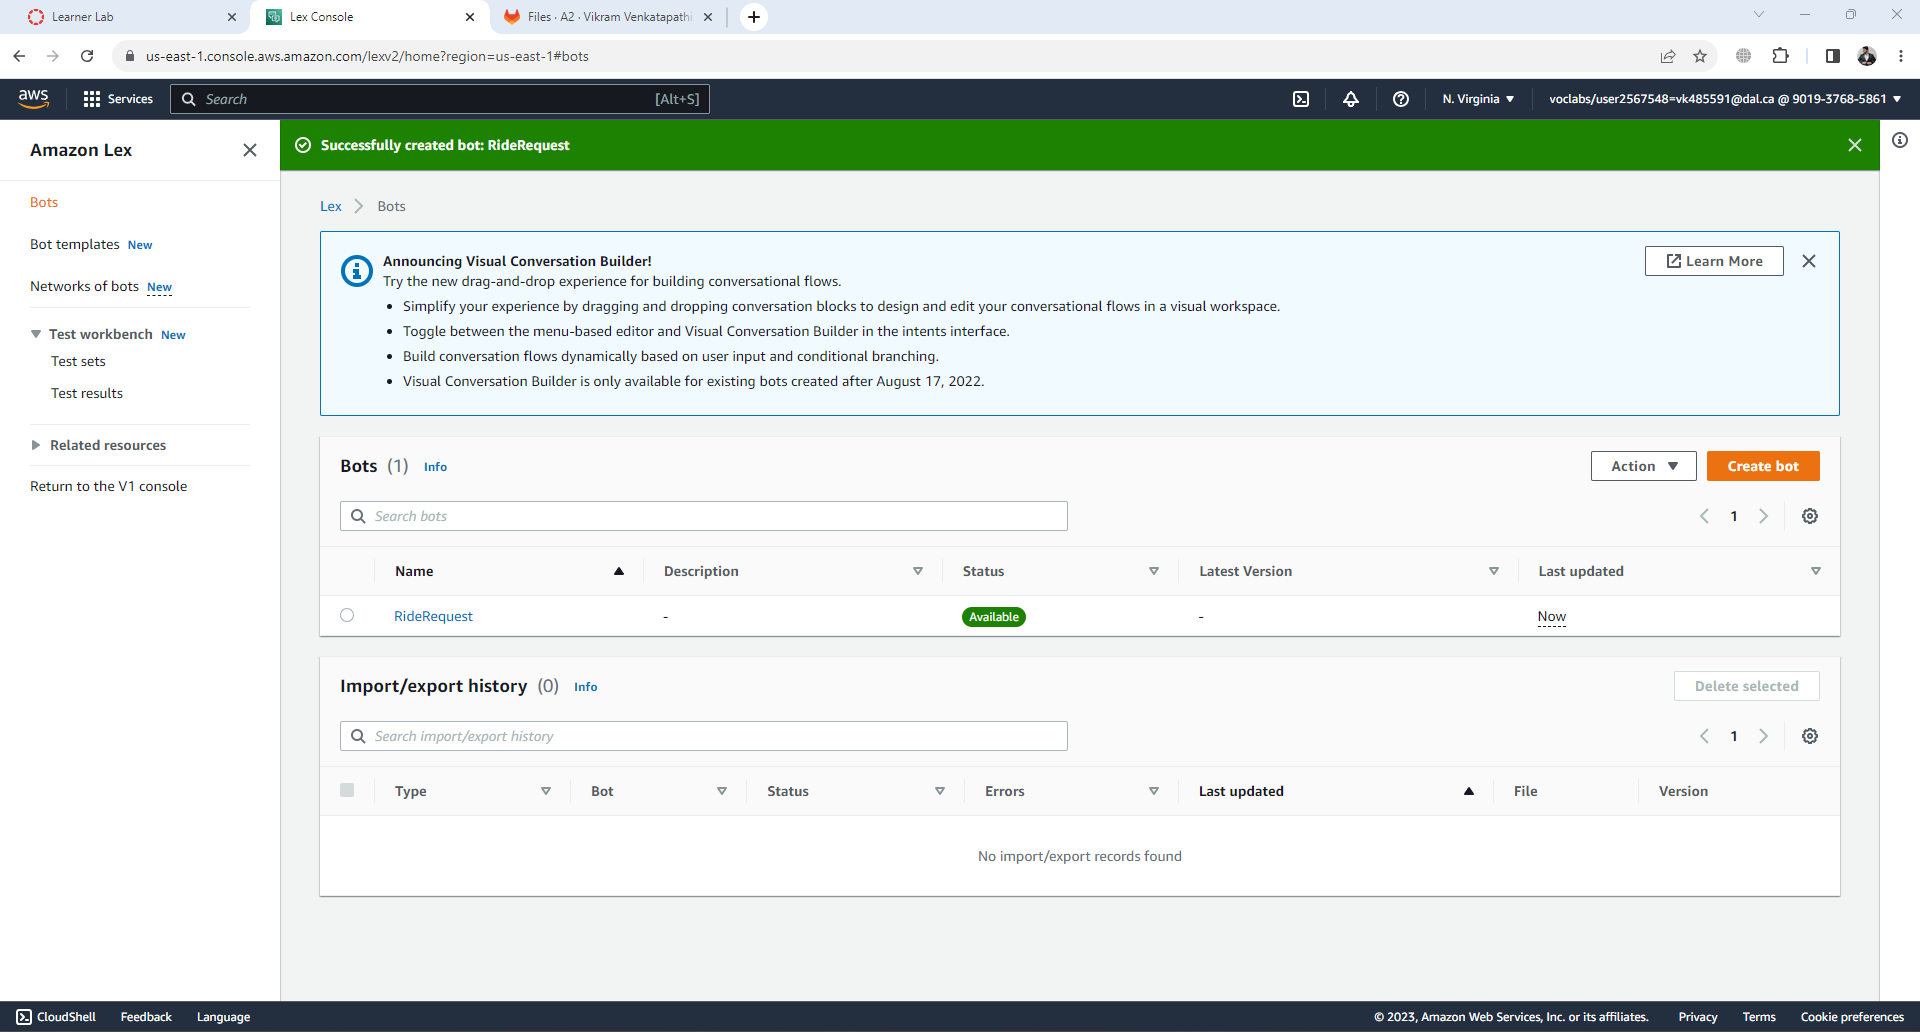
\includegraphics[scale=1, width=15cm,height=7.5cm]{PROBLEM 2/Screenshots/3. Lex/1.2 Bot created.png}}
    \caption{\textbf{\textit{Bot created}}}
    \label{fig:}
\end{figure}
\begin{figure}[htp]
    \centering
    \fbox{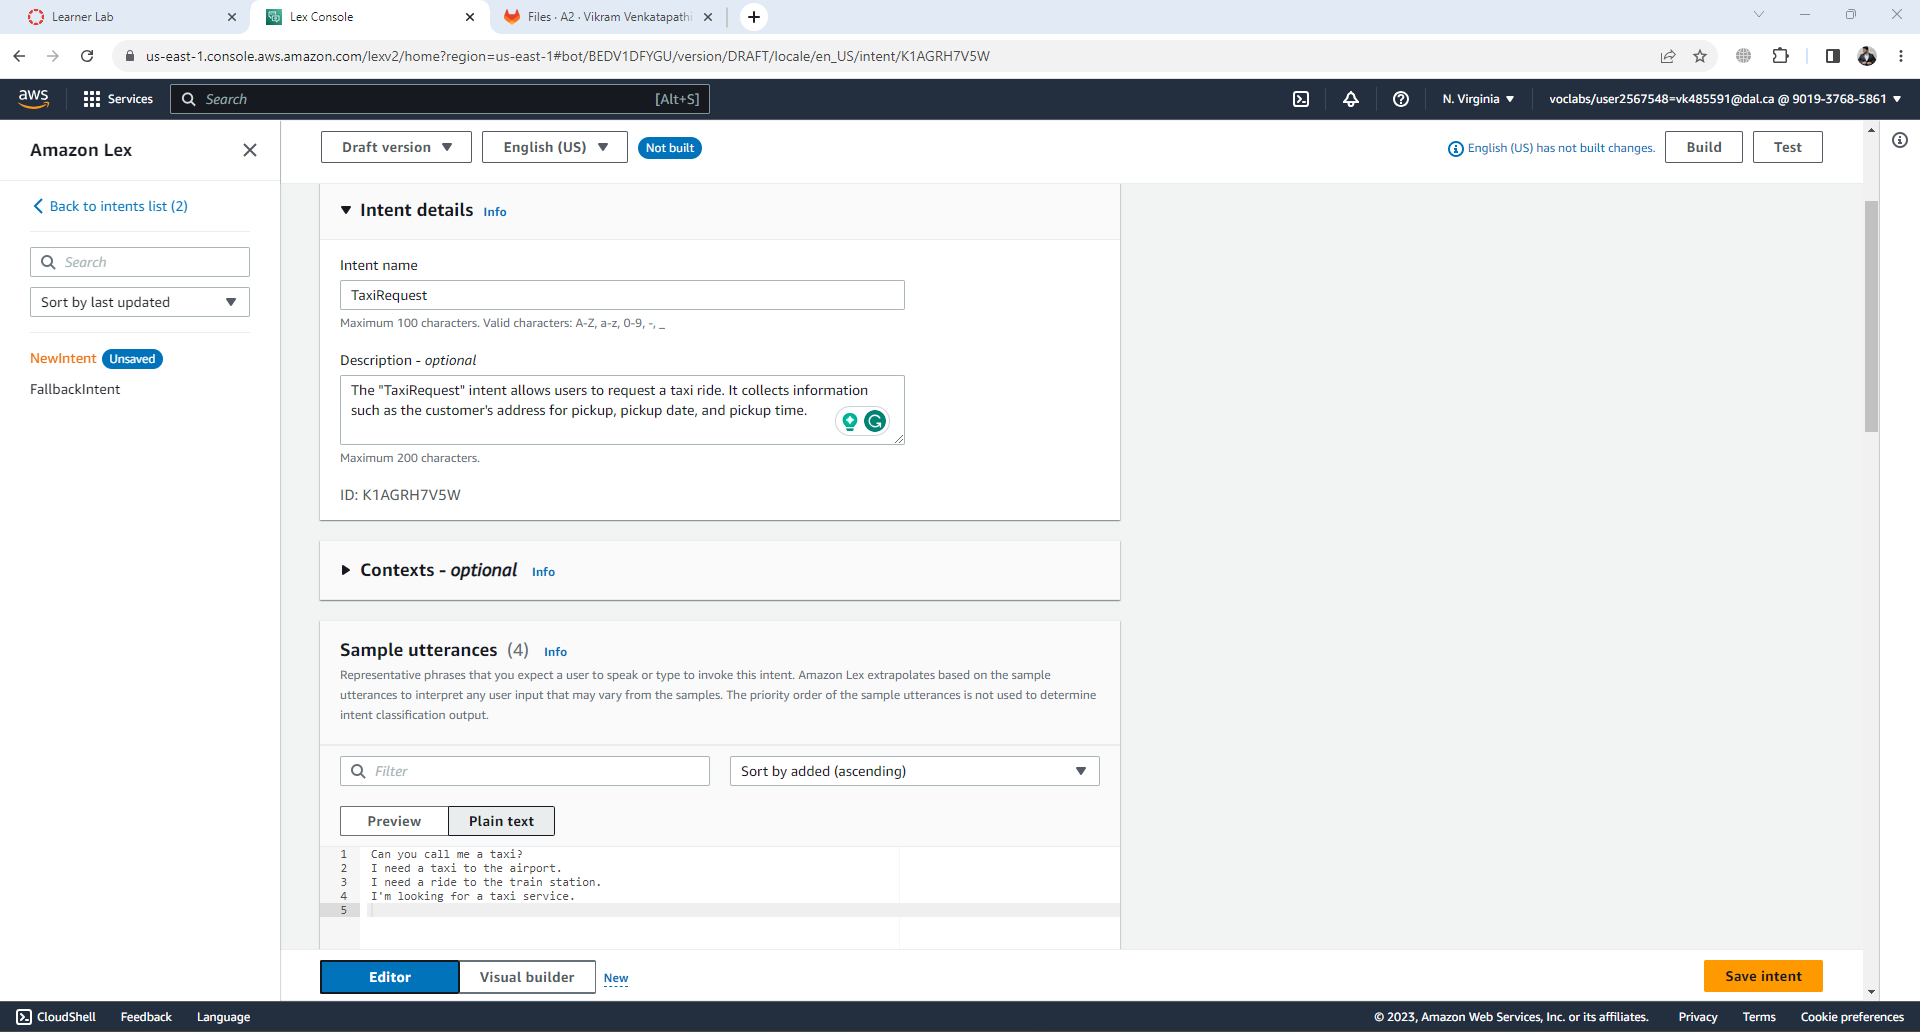
\includegraphics[scale=1, width=15cm,height=7.5cm]{PROBLEM 2/Screenshots/3. Lex/1. Taxi ride request/2.1 TaxiRequest intent creation.png}}
    \caption{\textbf{\textit{TaxiRequest intent creation}}}
    \label{fig:}
\end{figure}
\begin{figure}[htp]
    \centering
    \fbox{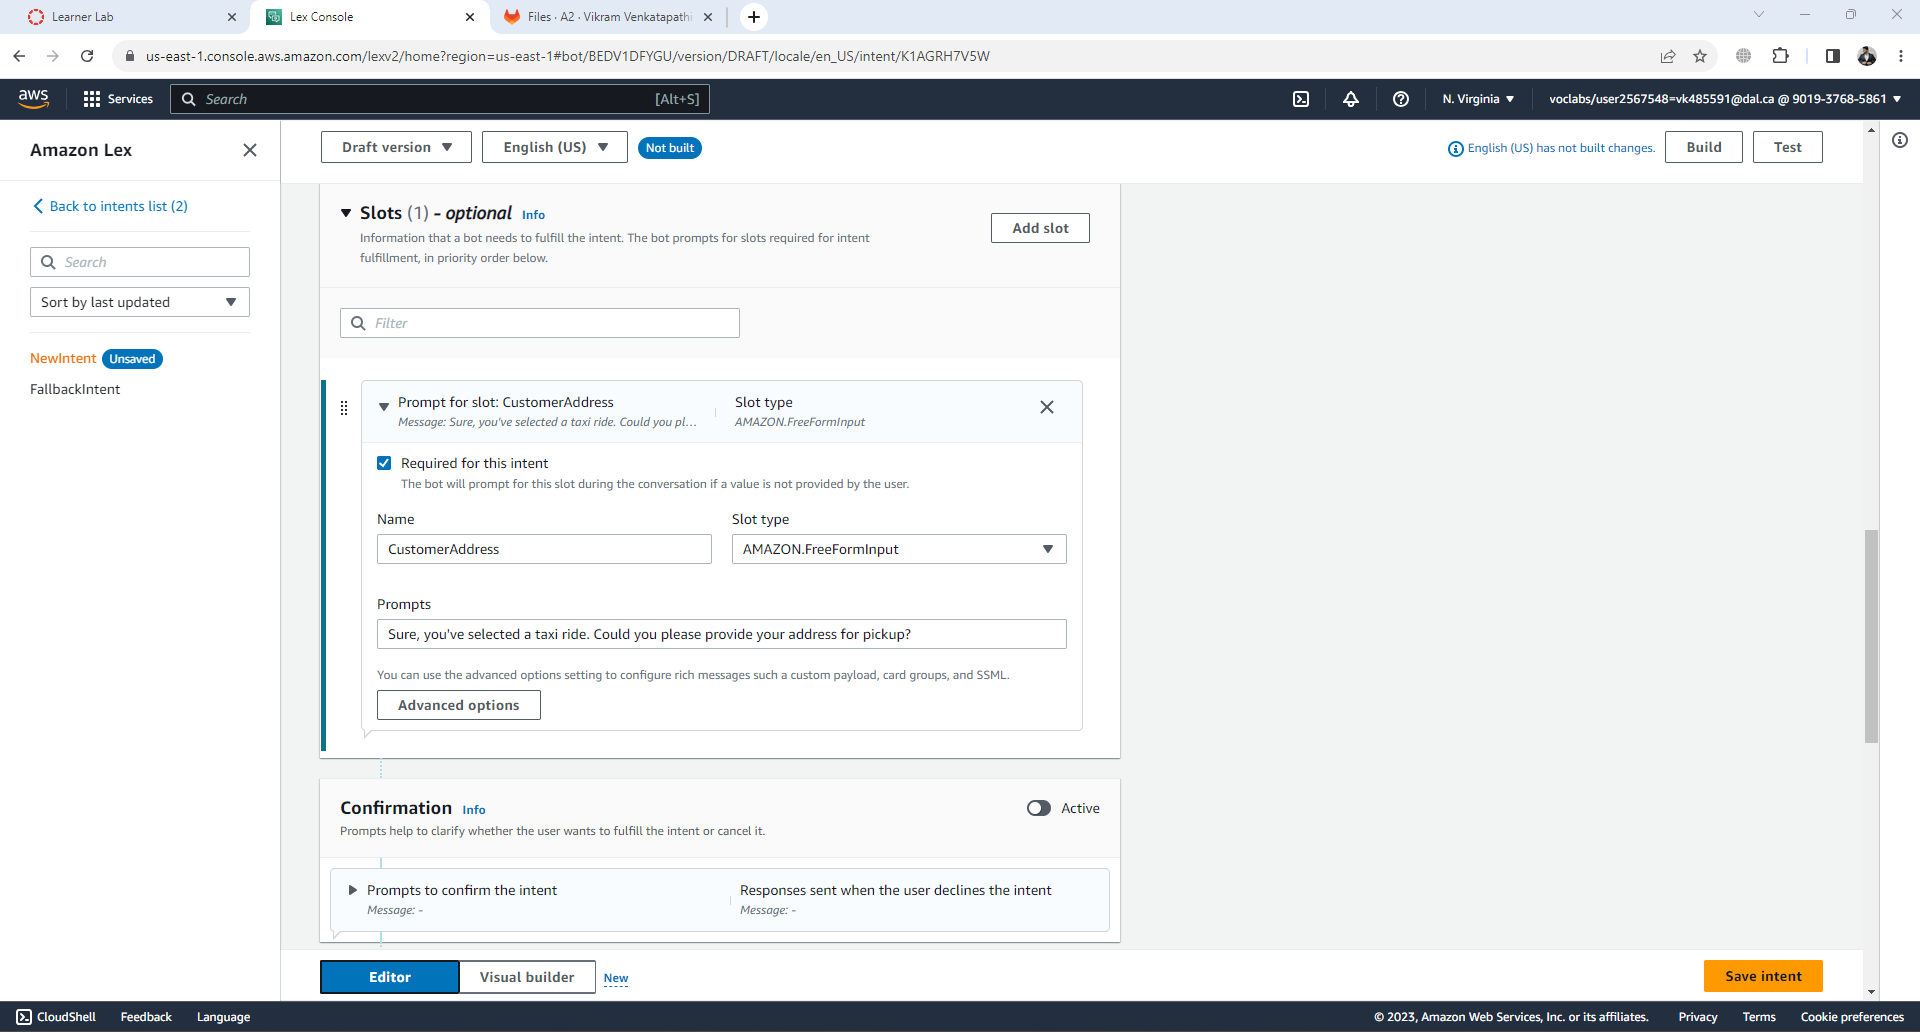
\includegraphics[scale=1, width=15cm,height=7.5cm]{PROBLEM 2/Screenshots/3. Lex/1. Taxi ride request/2.2 address slot.png}}
    \caption{\textbf{\textit{TaxiRequest intent creation - CustomerAddress slot}}}
    \label{fig:}
\end{figure}
\begin{figure}[htp]
    \centering
    \fbox{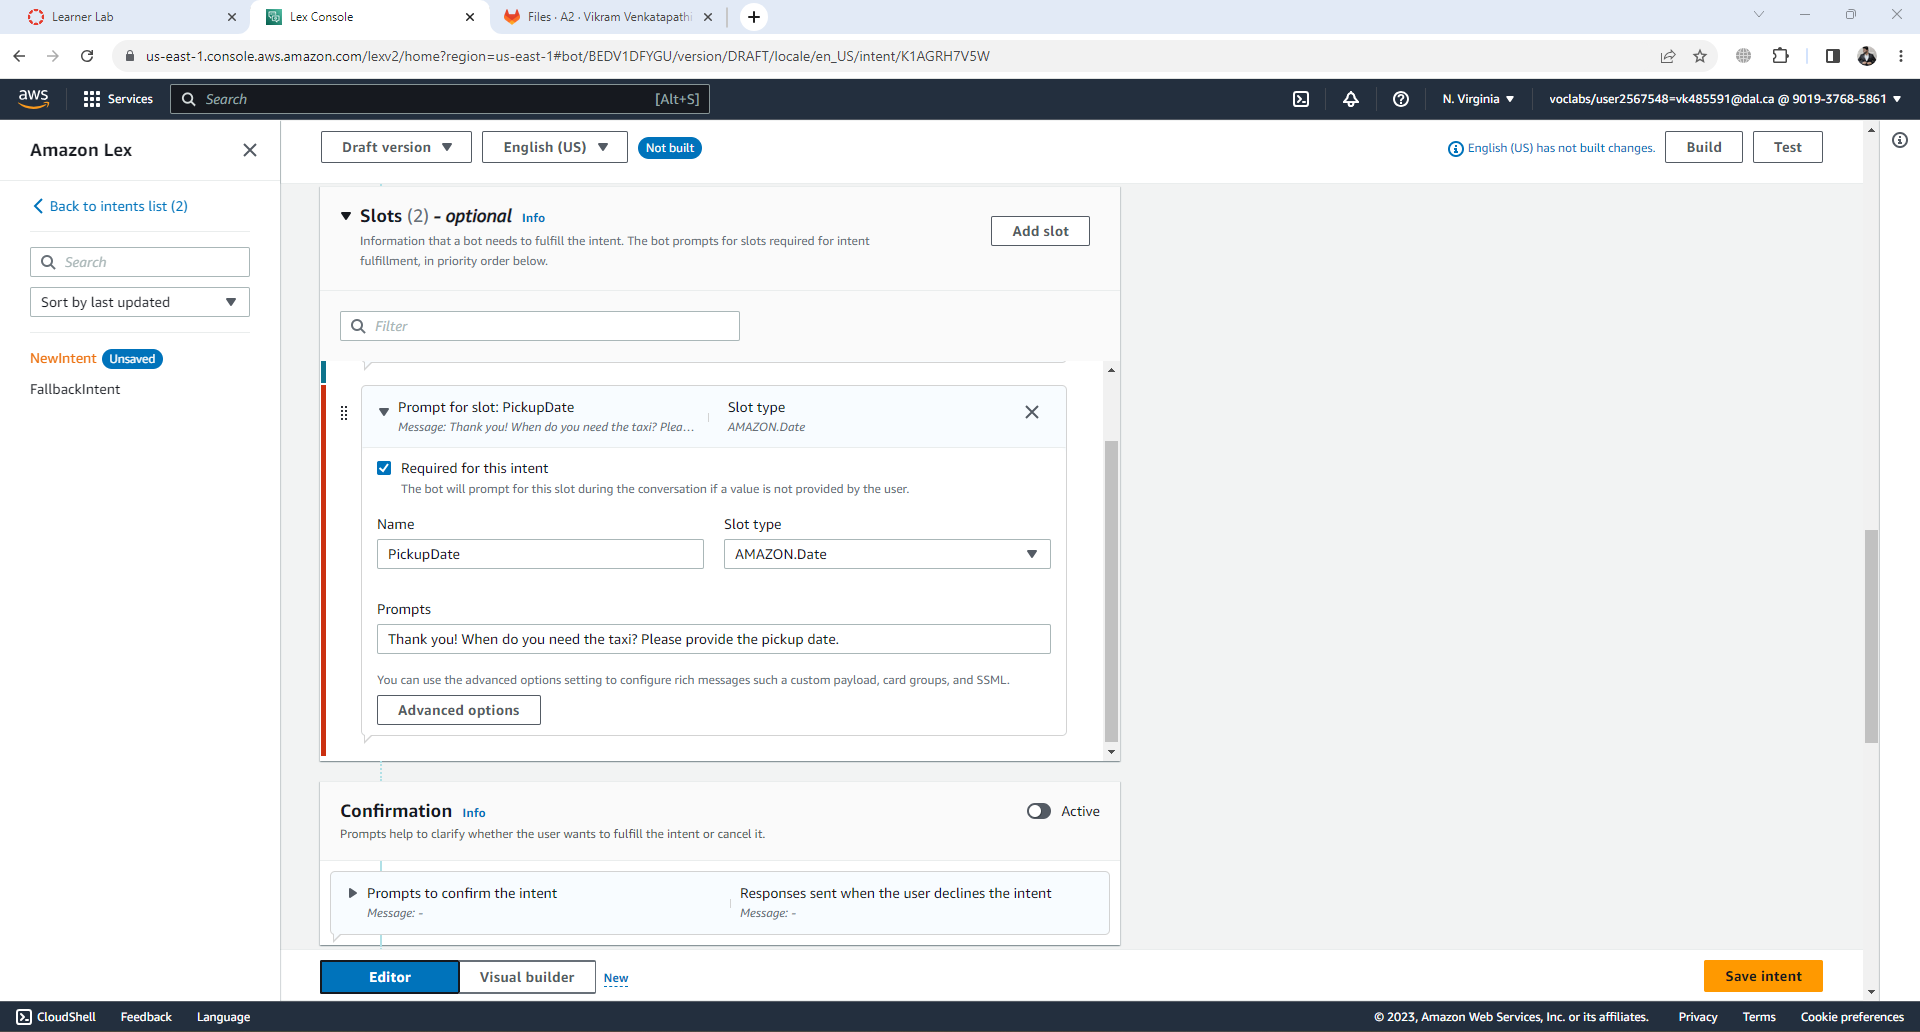
\includegraphics[scale=1, width=15cm,height=7.5cm]{PROBLEM 2/Screenshots/3. Lex/1. Taxi ride request/2.3 date slot.png}}
    \caption{\textbf{\textit{TaxiRequest intent creation - PickupDate slot}}}
    \label{fig:}
\end{figure}
\begin{figure}[htp]
    \centering
    \fbox{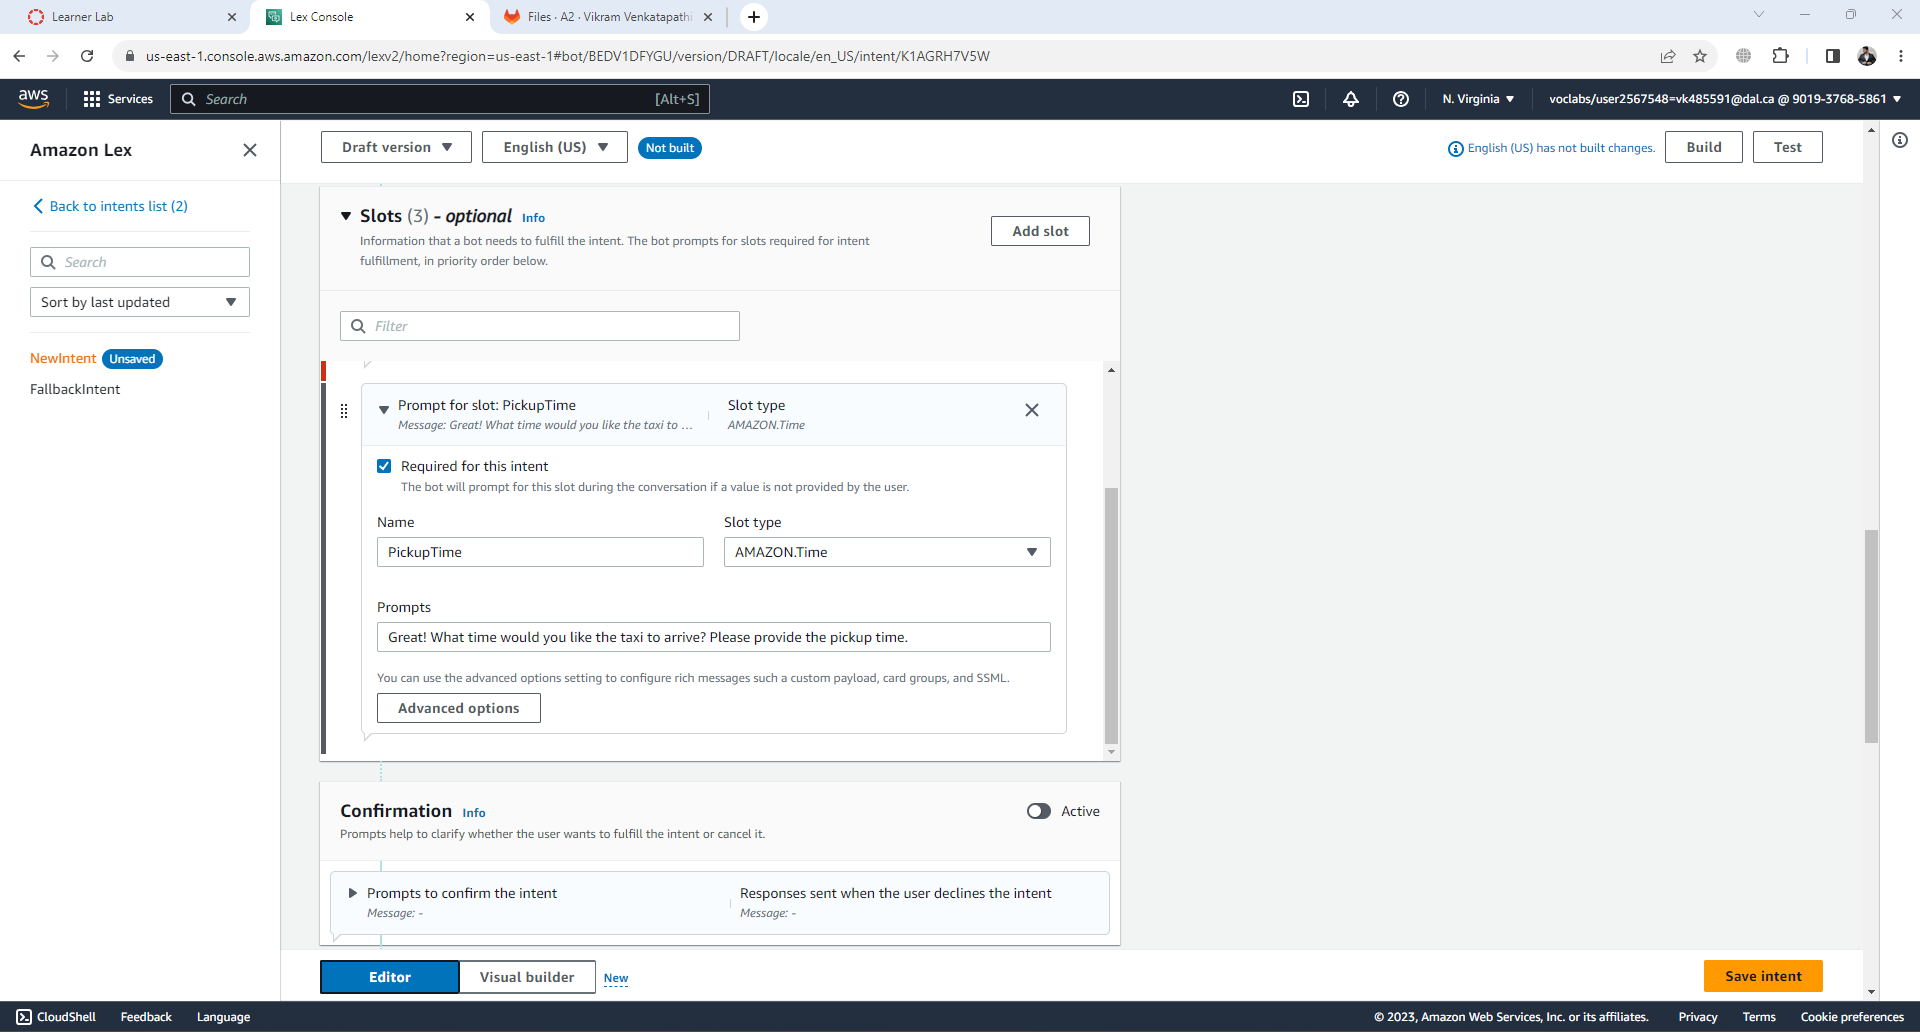
\includegraphics[scale=1, width=15cm,height=7.5cm]{PROBLEM 2/Screenshots/3. Lex/1. Taxi ride request/2.4 time slot.png}}
    \caption{\textbf{\textit{TaxiRequest intent creation - PickupTime slot}}}
    \label{fig:}
\end{figure}
\begin{figure}[htp]
    \centering
    \fbox{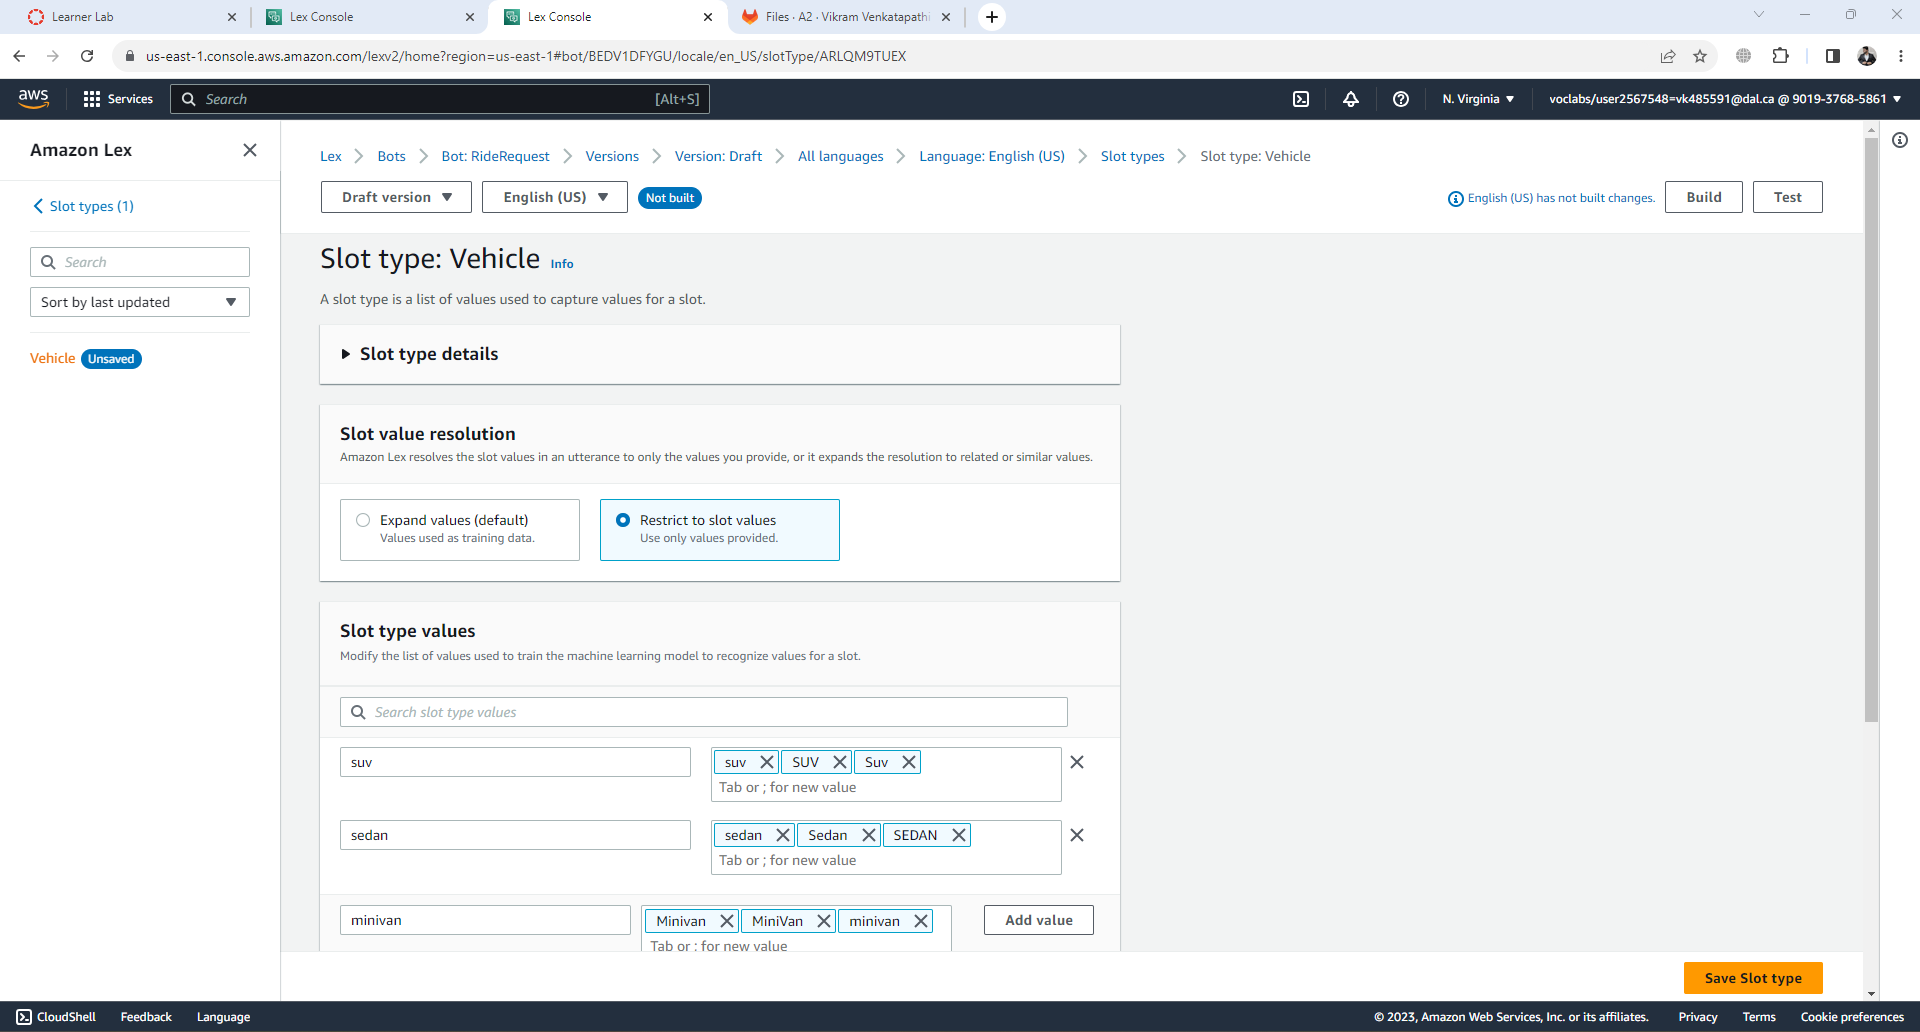
\includegraphics[scale=1, width=15cm,height=7.5cm]{PROBLEM 2/Screenshots/3. Lex/1. Taxi ride request/2.5 create slotype vehicle.png}}
    \caption{\textbf{\textit{TaxiRequest intent creation - Custom slot type 'Vehicle' creation}}}
    \label{fig:}
\end{figure}
\begin{figure}[htp]
    \centering
    \fbox{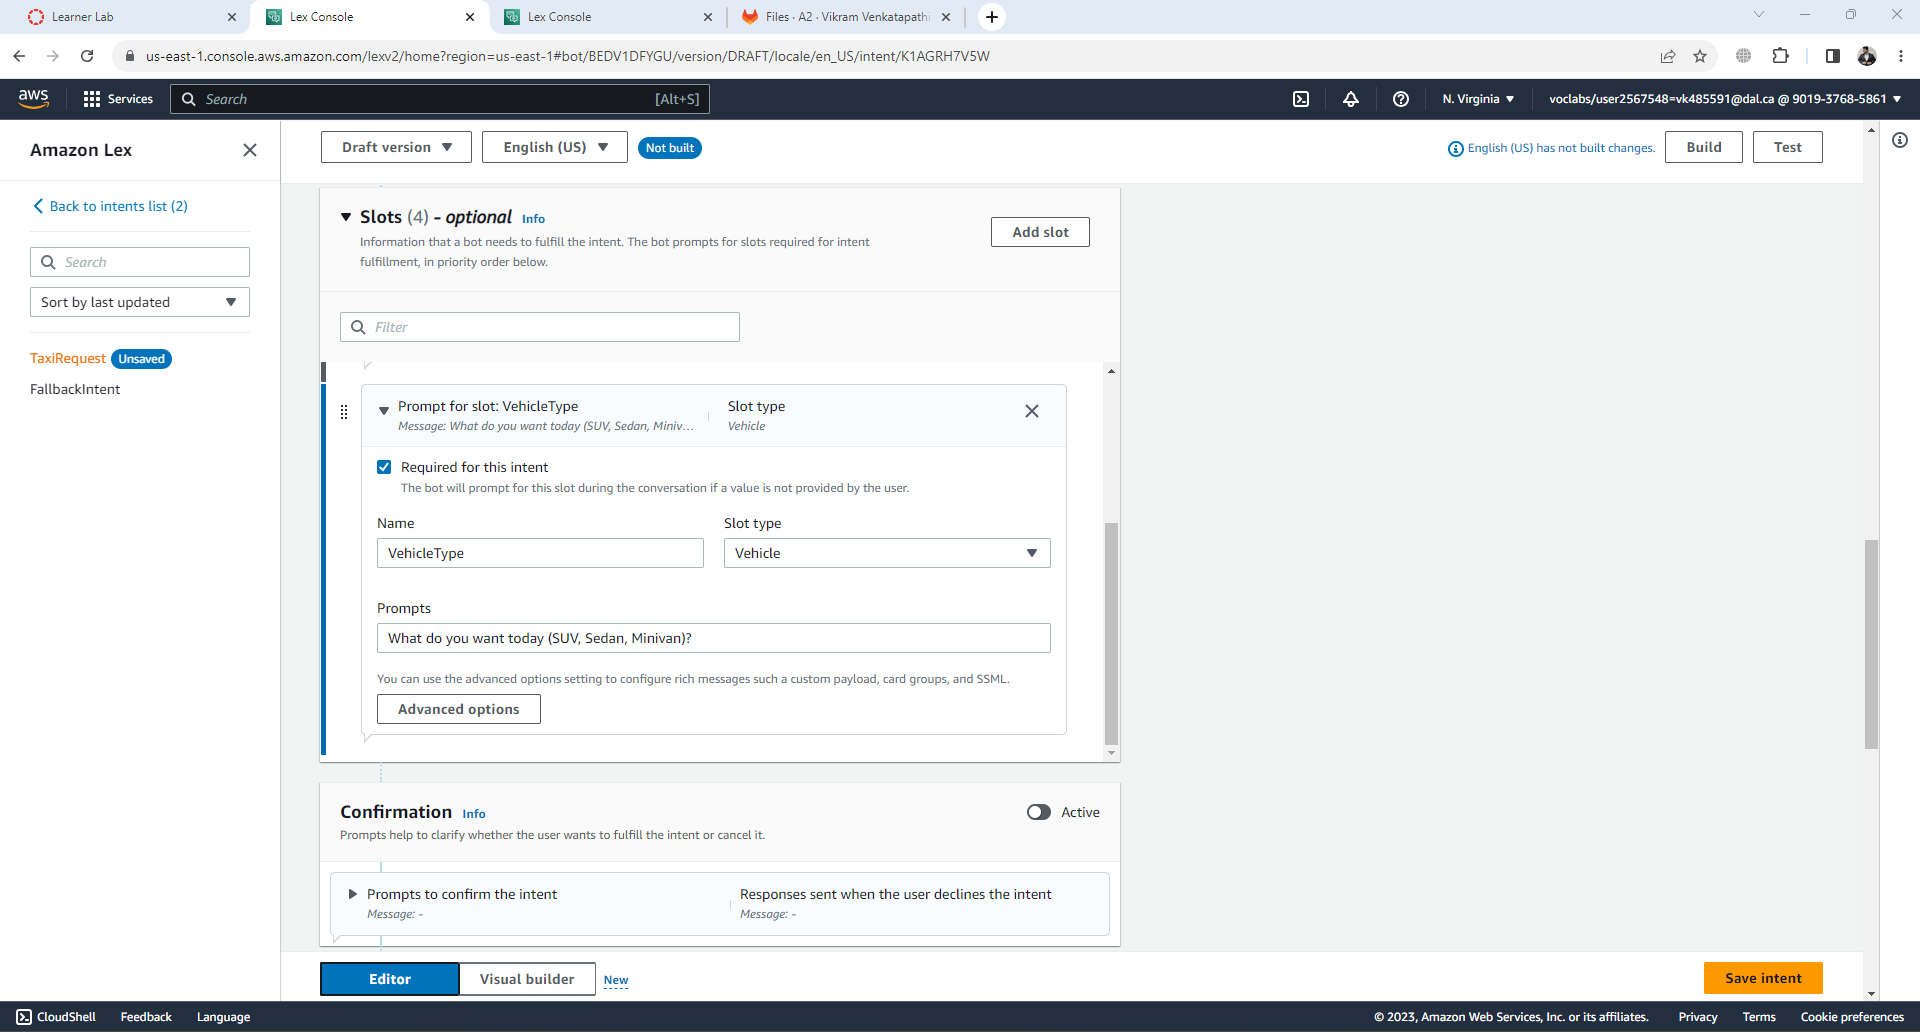
\includegraphics[scale=1, width=15cm,height=7.5cm]{PROBLEM 2/Screenshots/3. Lex/1. Taxi ride request/2.6 vechicle type slot.png}}
    \caption{\textbf{\textit{TaxiRequest intent creation - VechicleType slot}}}
    \label{fig:}
\end{figure}
\begin{figure}[htp]
    \centering
    \fbox{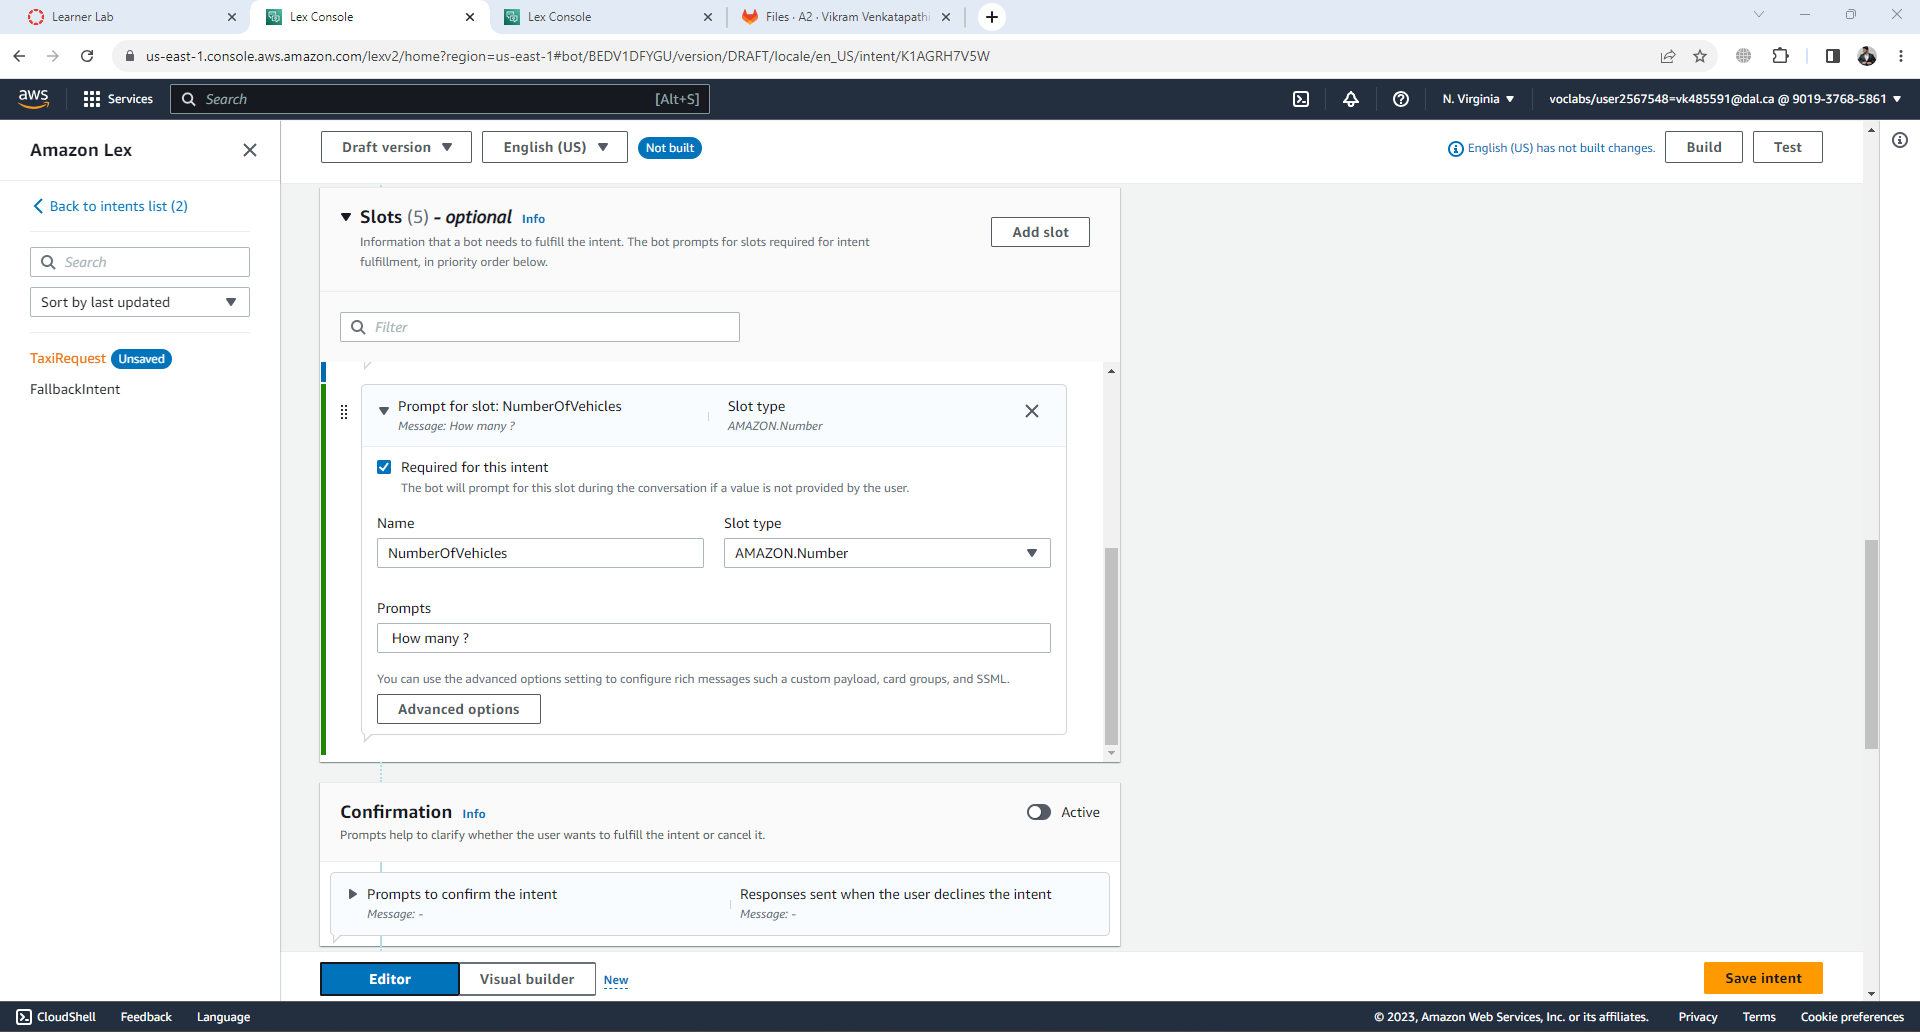
\includegraphics[scale=1, width=15cm,height=7.5cm]{PROBLEM 2/Screenshots/3. Lex/1. Taxi ride request/2.7 no. of vehicles slot.png}}
    \caption{\textbf{\textit{TaxiRequest intent creation - NumberOfVehicles slot}}}
    \label{fig:}
\end{figure}
\begin{figure}[htp]
    \centering
    \fbox{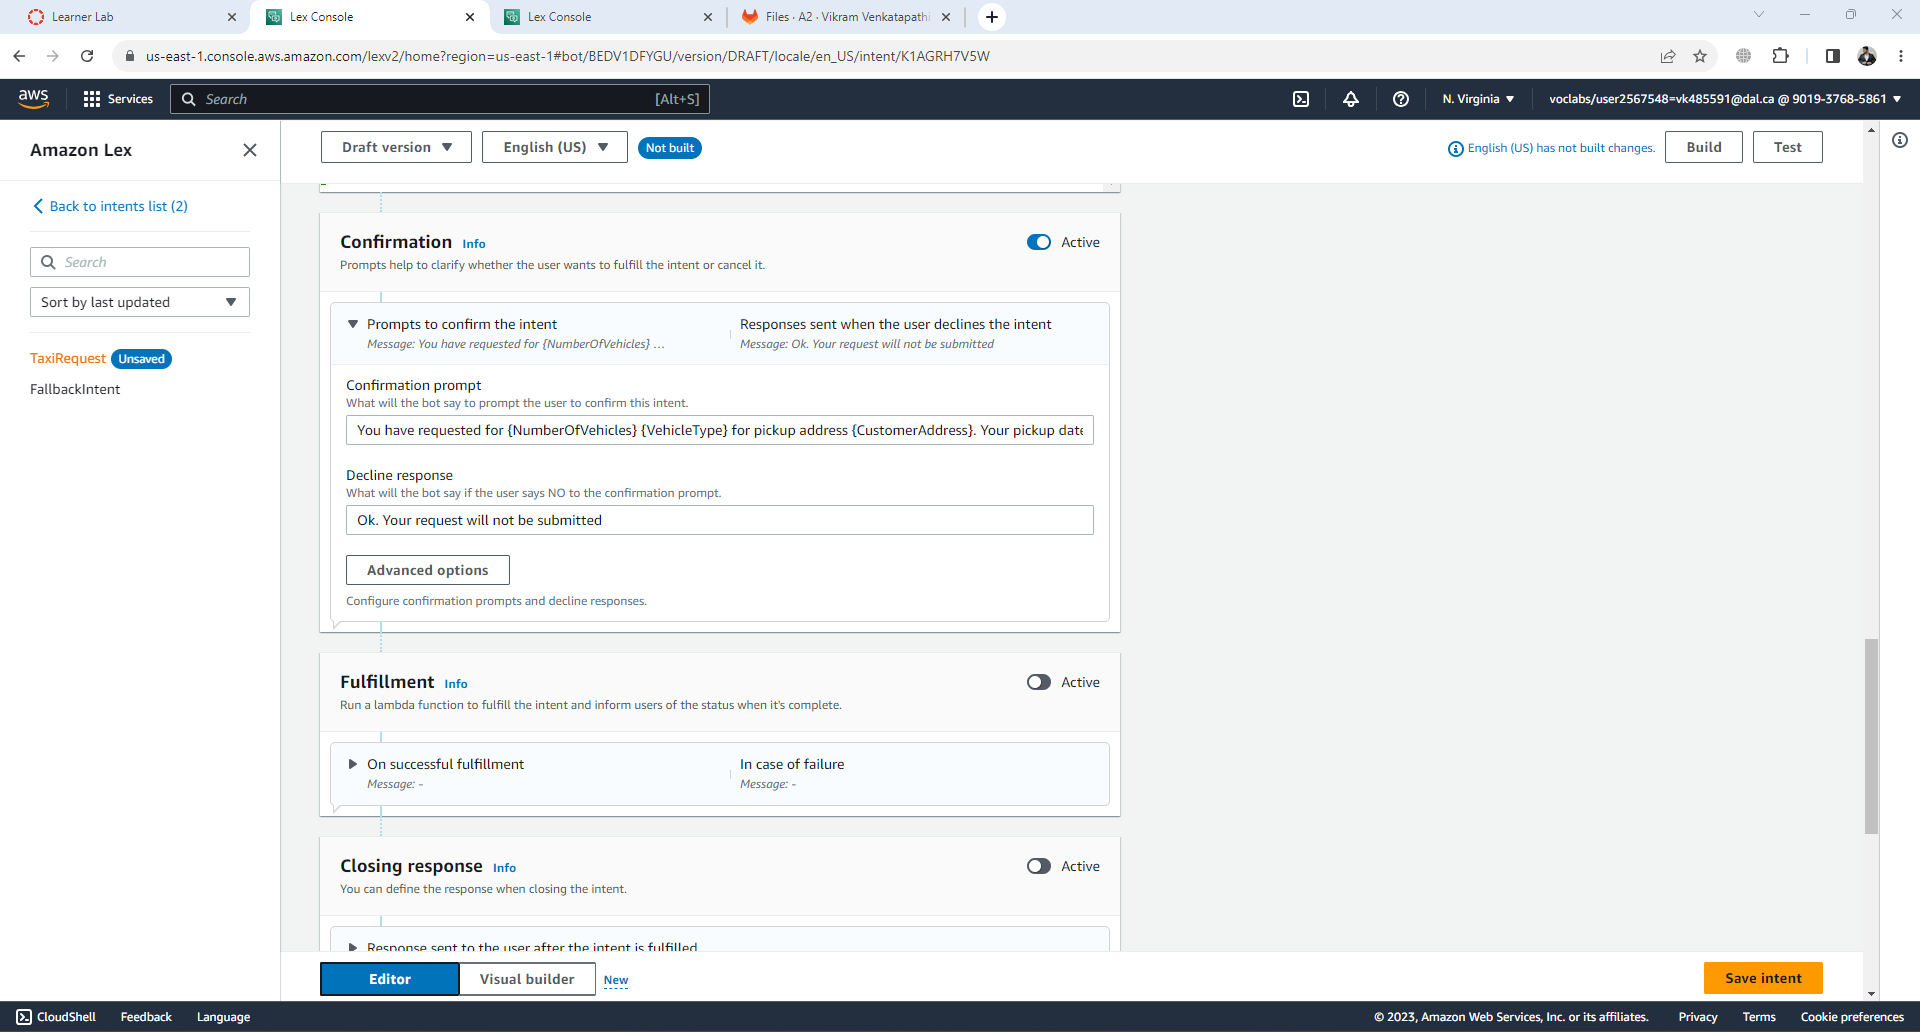
\includegraphics[scale=1, width=15cm,height=7.5cm]{PROBLEM 2/Screenshots/3. Lex/1. Taxi ride request/2.8 add confirmation prompt.png}}
    \caption{\textbf{\textit{TaxiRequest intent creation - Add Confirmation prompt with placeholder values}}}
    \label{fig:}
\end{figure}
\begin{figure}[htp]
    \centering
    \fbox{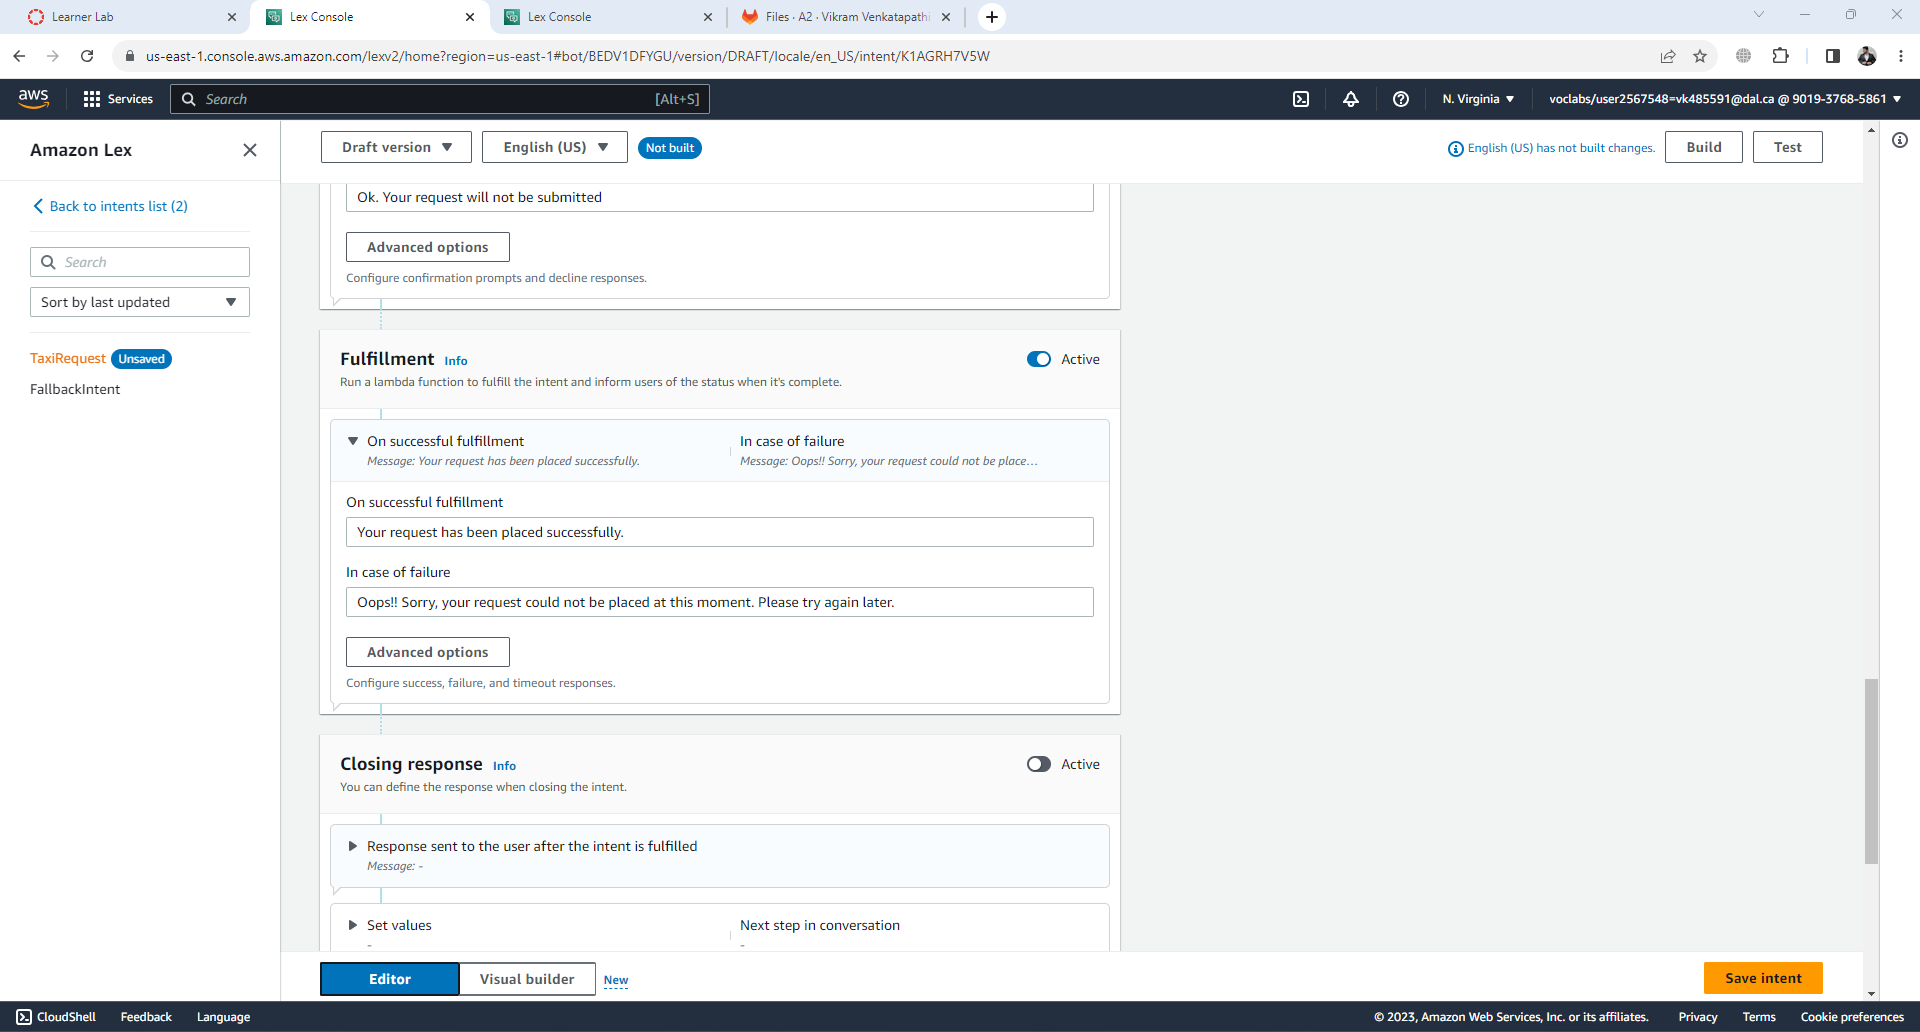
\includegraphics[scale=1, width=15cm,height=7.5cm]{PROBLEM 2/Screenshots/3. Lex/1. Taxi ride request/2.9 fullfilment prompt.png}}
    \caption{\textbf{\textit{TaxiRequest intent creation - Add fullfillment prompt}}}
    \label{fig:}
\end{figure}
\begin{figure}[htp]
    \centering
    \fbox{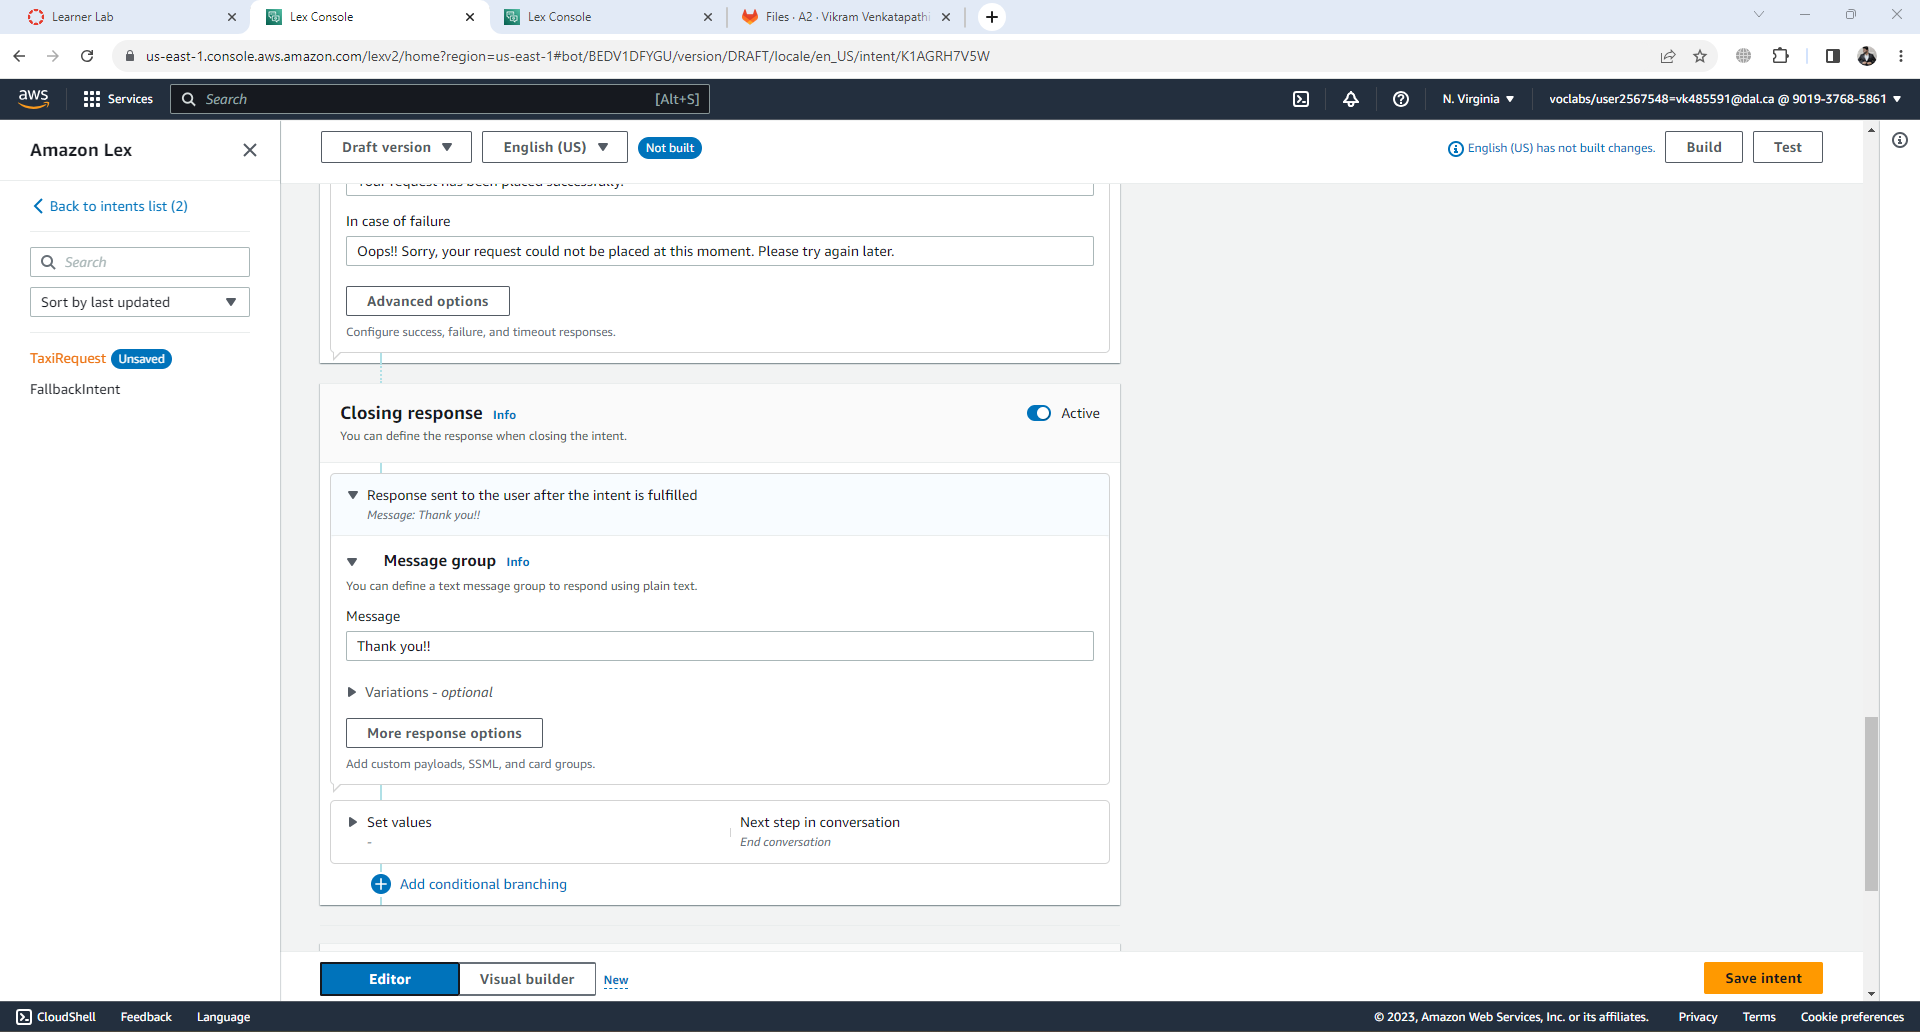
\includegraphics[scale=1, width=15cm,height=7.5cm]{PROBLEM 2/Screenshots/3. Lex/1. Taxi ride request/2.10 add closing response.png}}
    \caption{\textbf{\textit{TaxiRequest intent creation - Add closing response}}}
    \label{fig:}
\end{figure}

\begin{figure}[htp]
    \centering
    \fbox{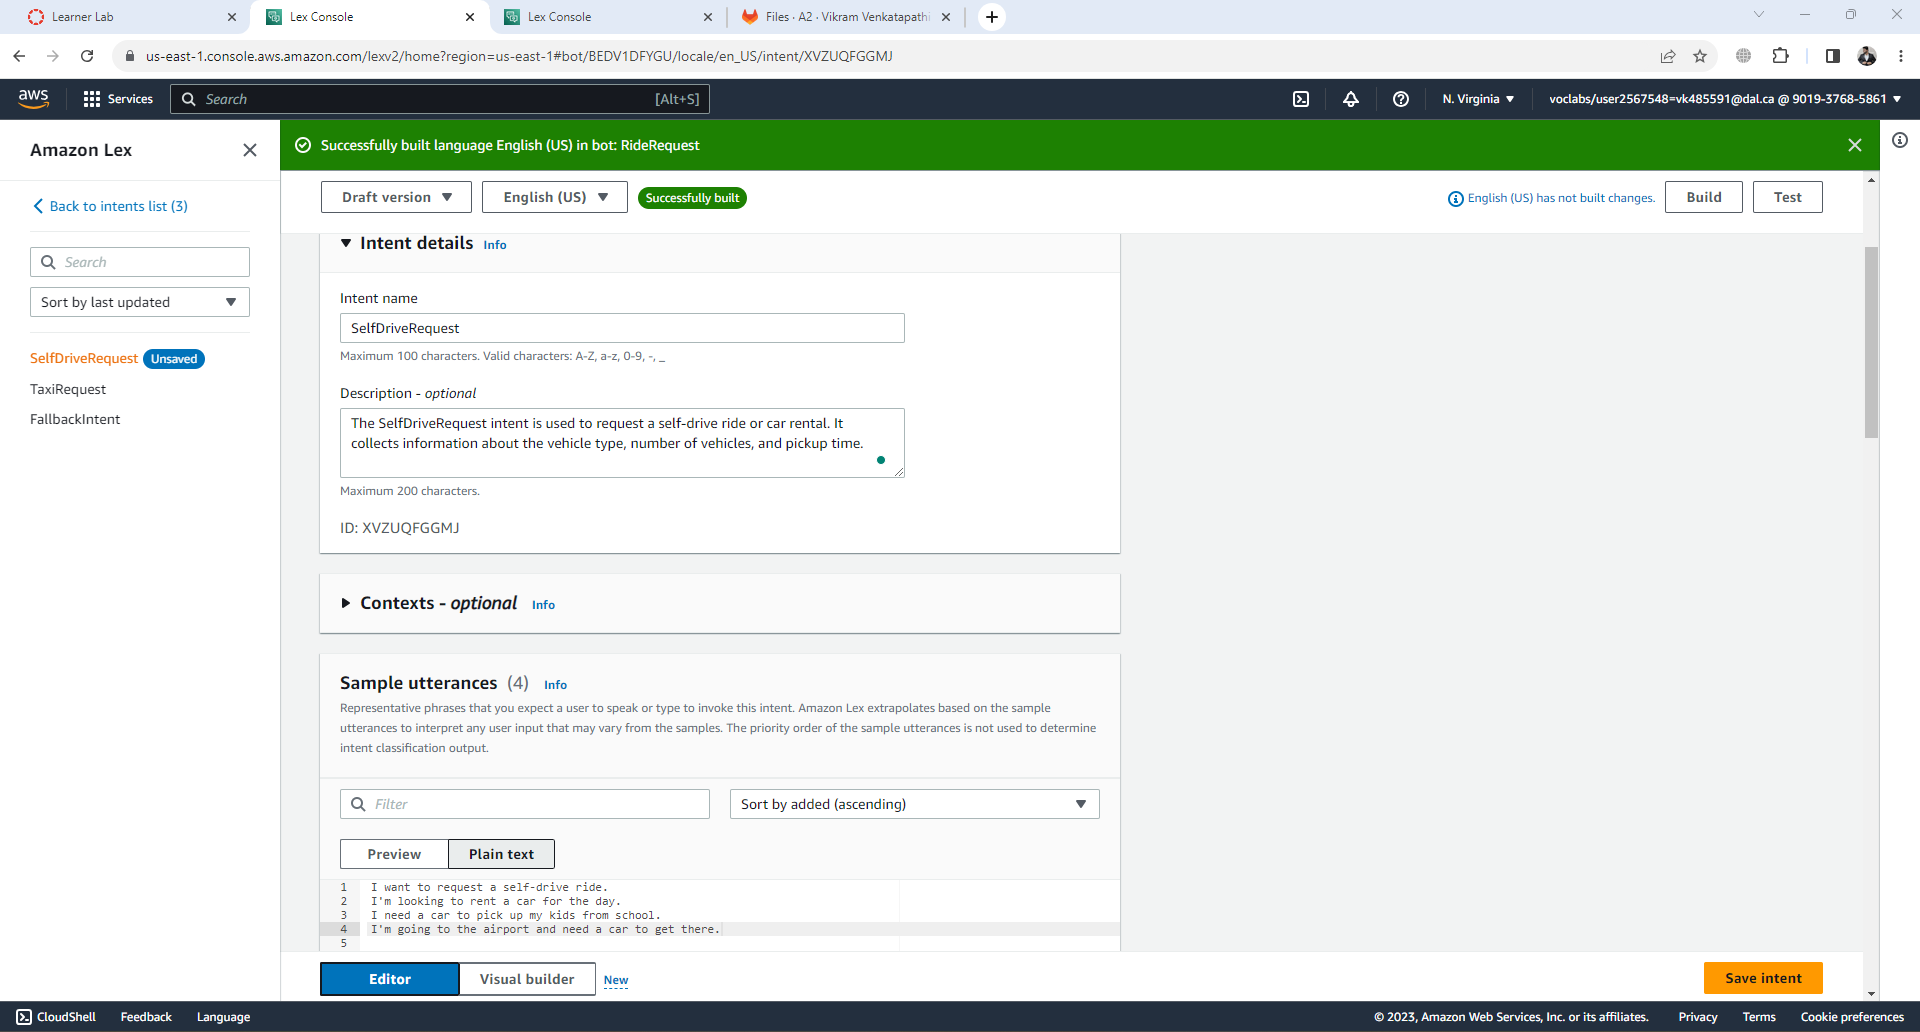
\includegraphics[scale=1, width=15cm,height=7.5cm]{PROBLEM 2/Screenshots/3. Lex/2. Self ride request/3.1 SelfDriveRequest intent creation.png}}
    \caption{\textbf{\textit{SelfDriveRequest intent creation}}}
    \label{fig:}
\end{figure}

\begin{figure}[htp]
    \centering
    \fbox{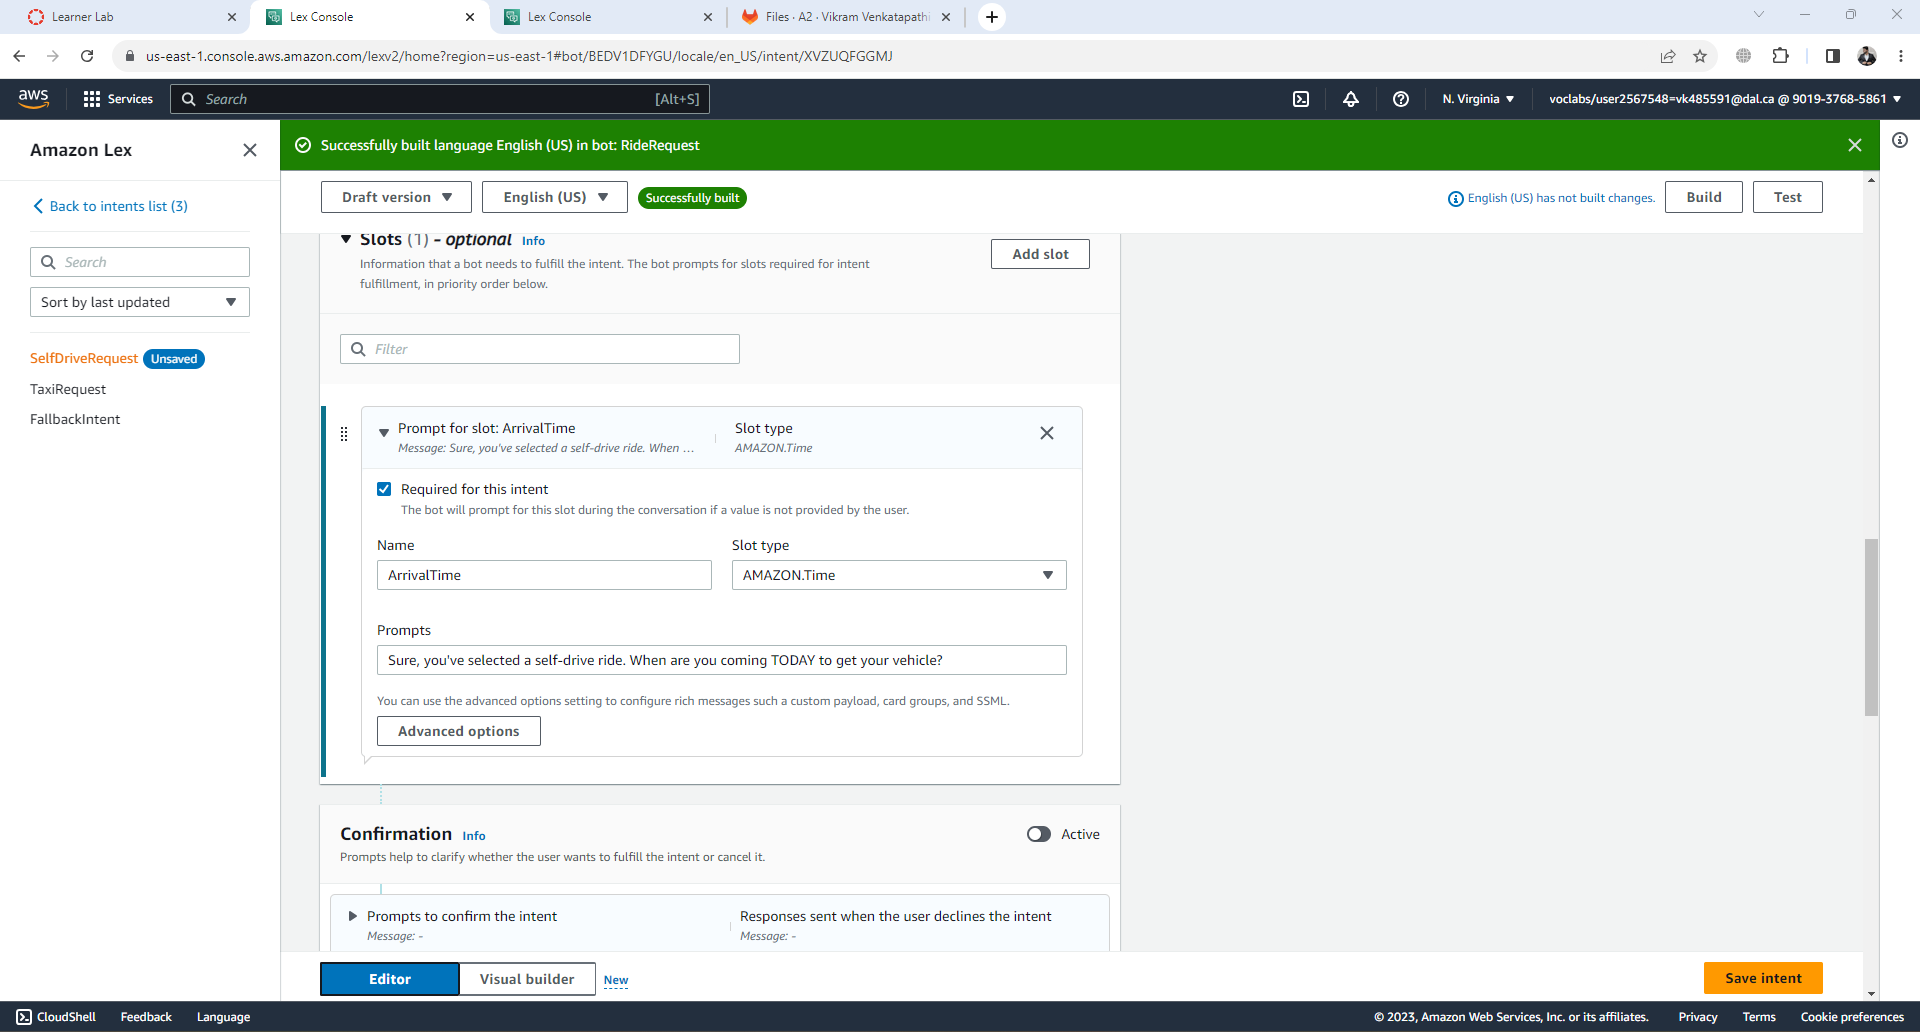
\includegraphics[scale=1, width=15cm,height=7.5cm]{PROBLEM 2/Screenshots/3. Lex/2. Self ride request/3.2 arrival time slot.png}}
    \caption{\textbf{\textit{SelfDriveRequest intent creation - ArrivalTime slot}}}
    \label{fig:}
\end{figure}
\begin{figure}[htp]
    \centering
    \fbox{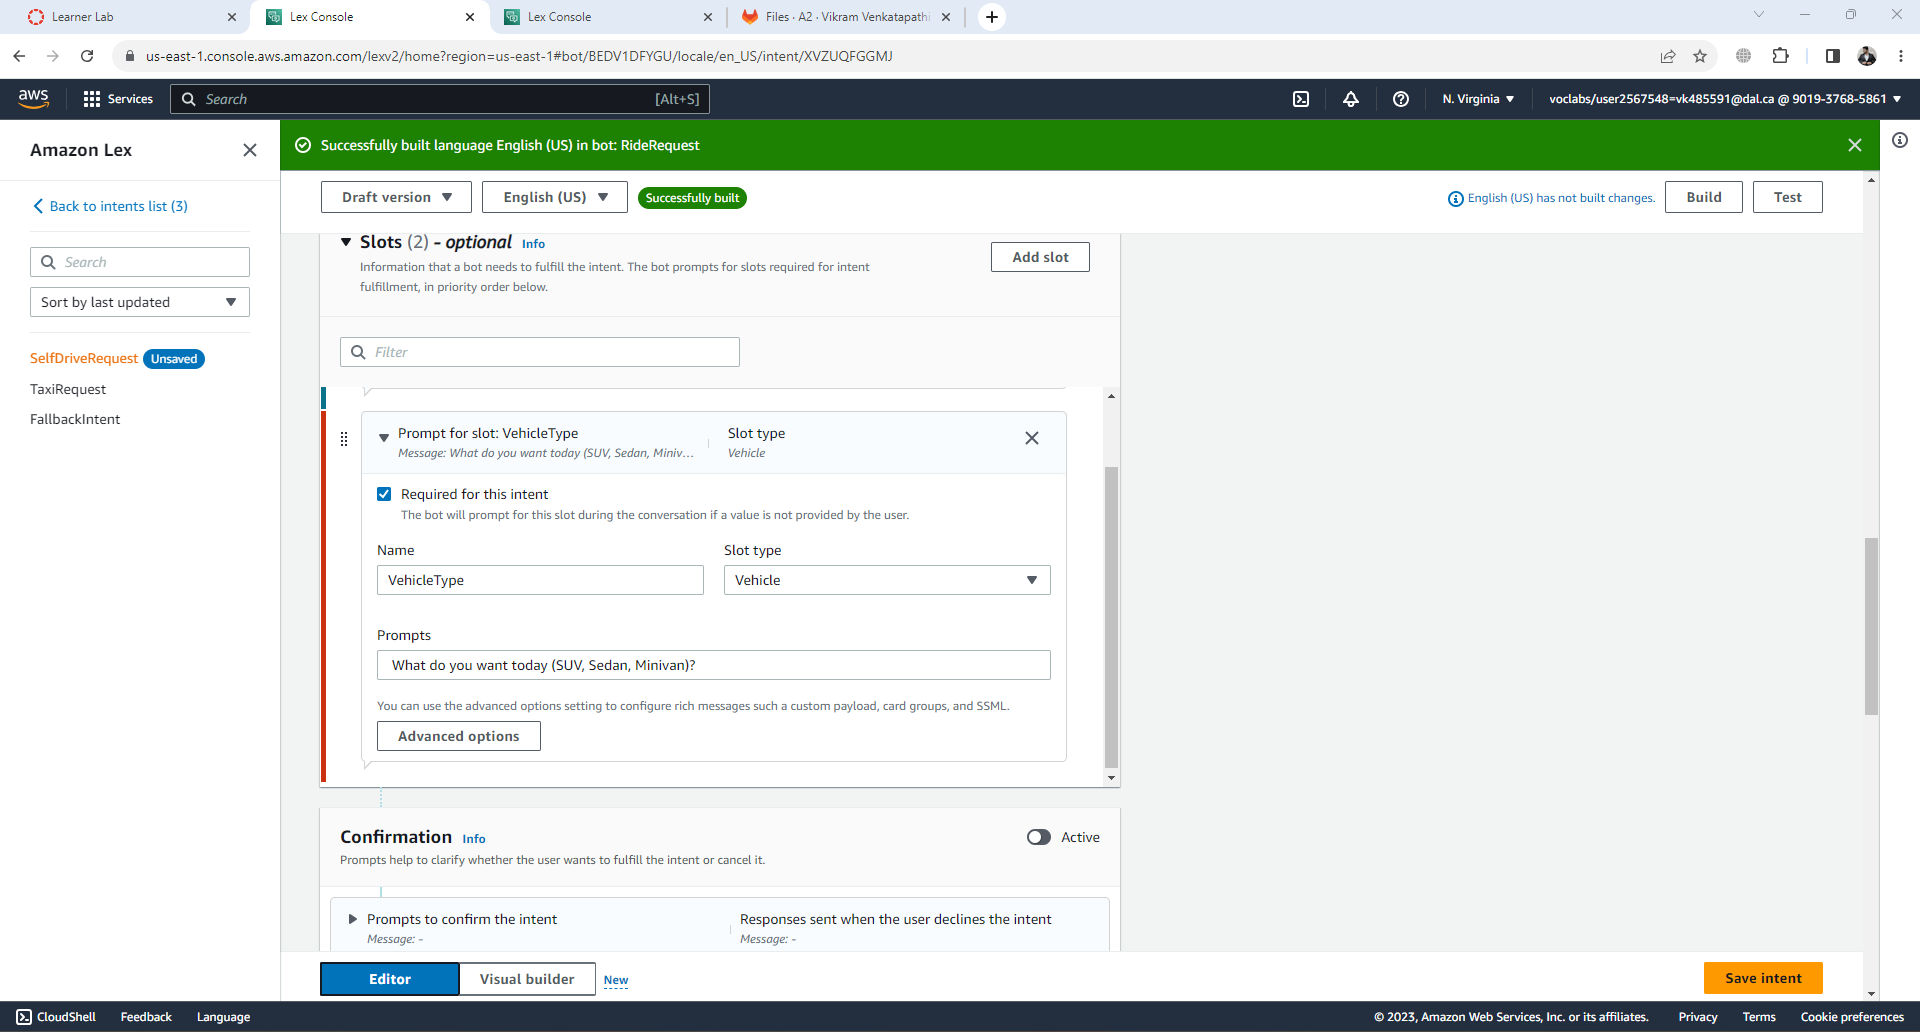
\includegraphics[scale=1, width=15cm,height=7.5cm]{PROBLEM 2/Screenshots/3. Lex/2. Self ride request/3.3 vehicle type slot.png}}
    \caption{\textbf{\textit{SelfDriveRequest intent creation - VehicleType slot}}}
    \label{fig:}
\end{figure}
\begin{figure}[htp]
    \centering
    \fbox{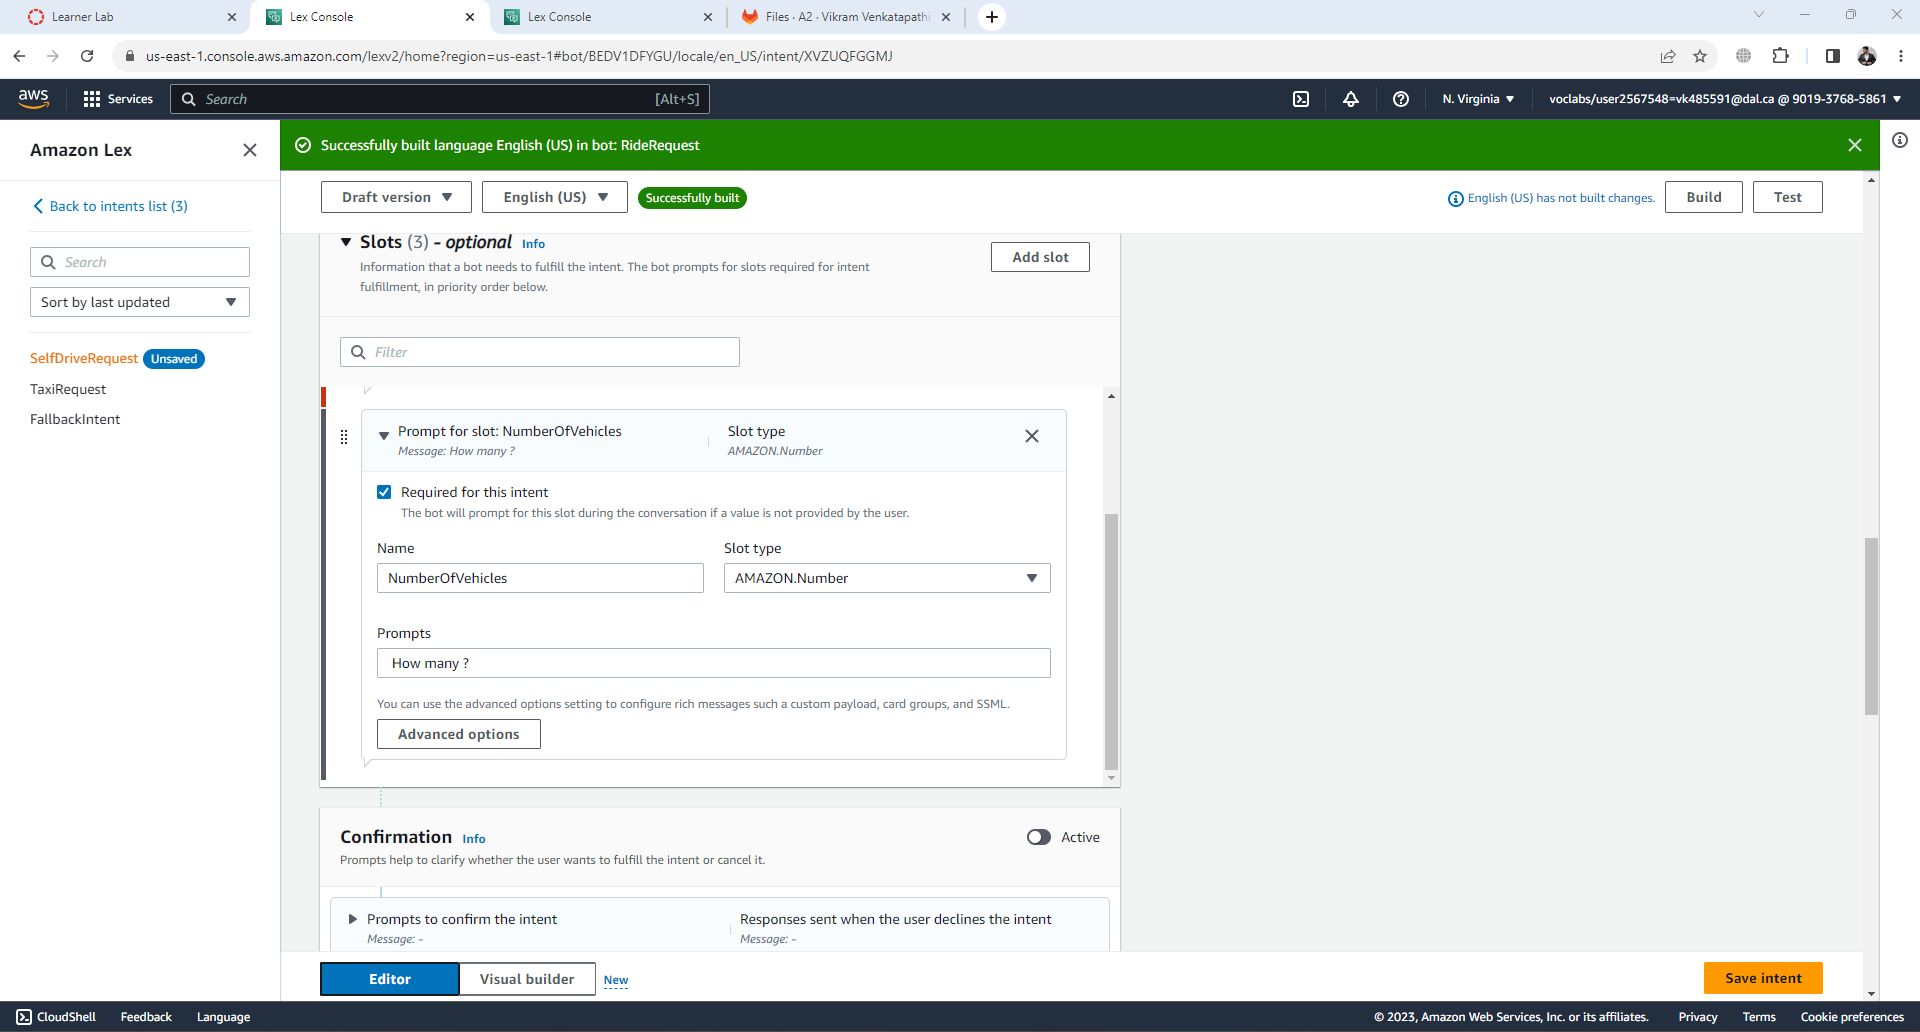
\includegraphics[scale=1, width=15cm,height=7.5cm]{PROBLEM 2/Screenshots/3. Lex/2. Self ride request/3.4 no. of vehicles slot.png}}
    \caption{\textbf{\textit{SelfDriveRequest intent creation - NumberOfVehicles slot}}}
    \label{fig:}
\end{figure}
\begin{figure}[htp]
    \centering
    \fbox{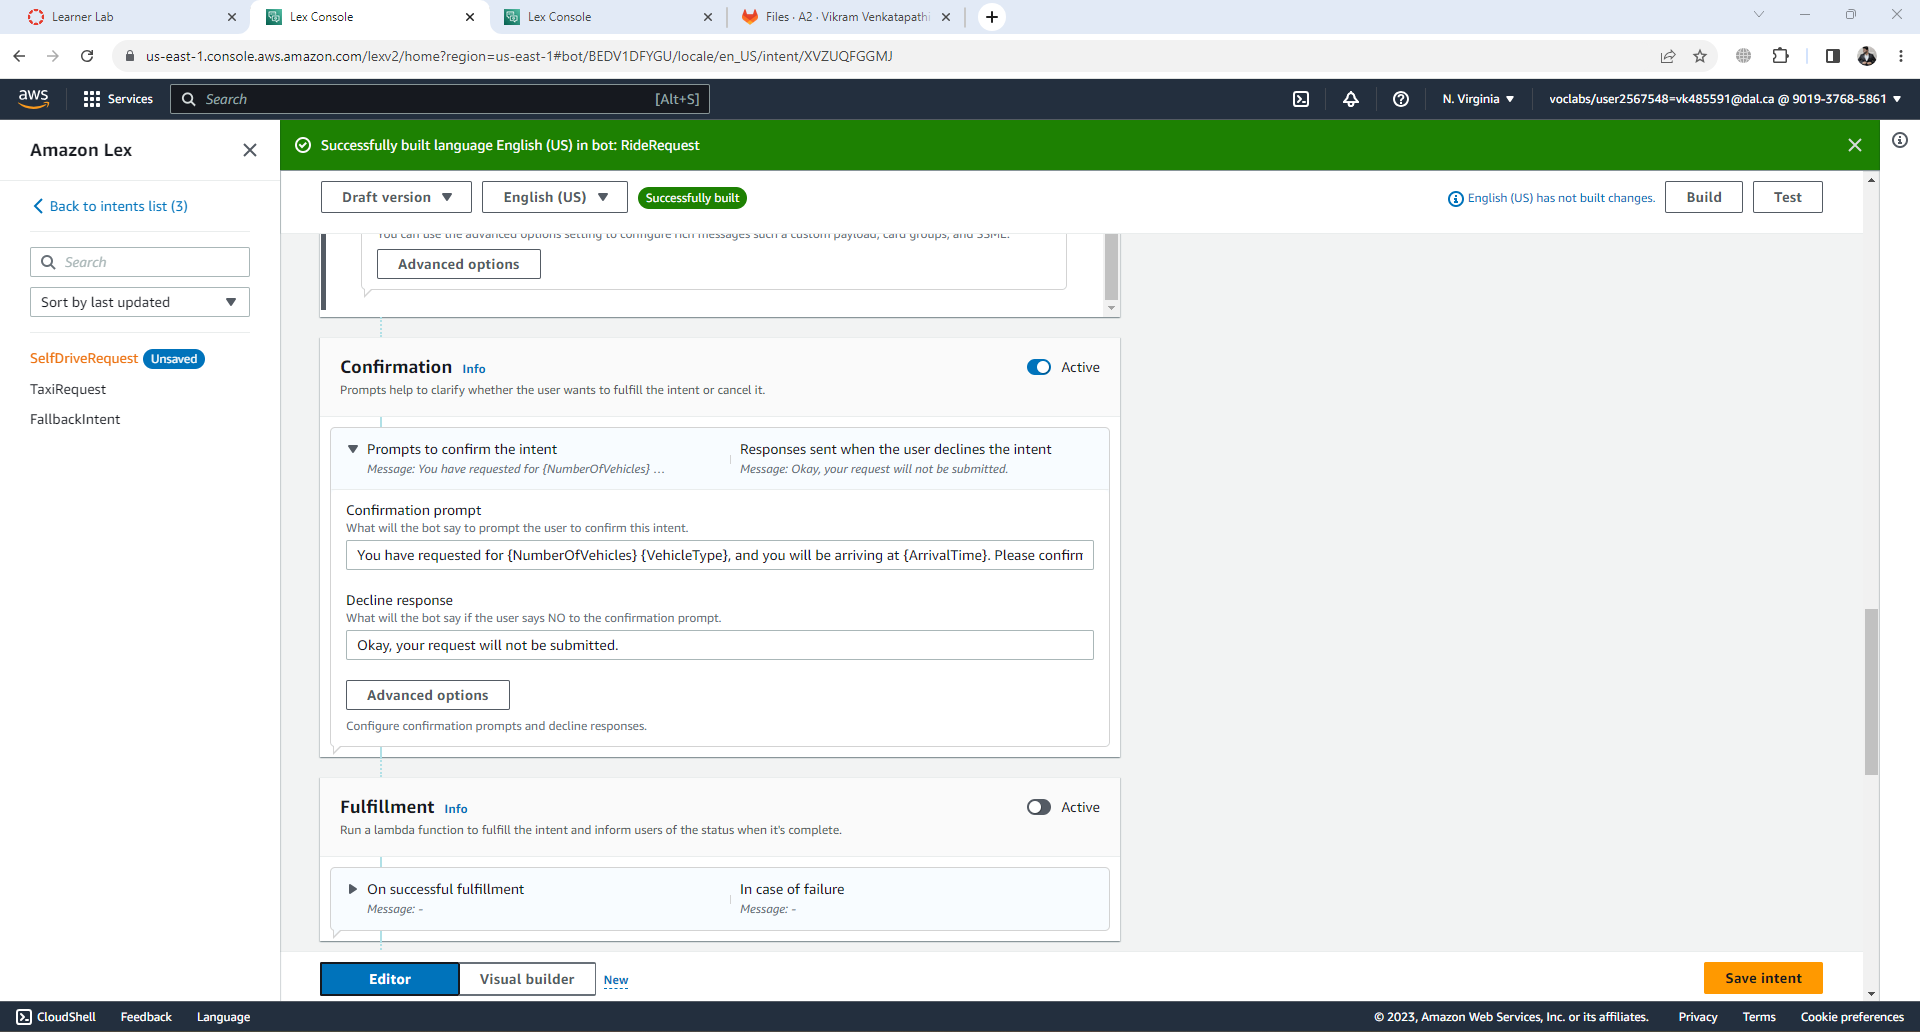
\includegraphics[scale=1, width=15cm,height=7.5cm]{PROBLEM 2/Screenshots/3. Lex/2. Self ride request/3.5 confirmation prompt.png}}
    \caption{\textbf{\textit{SelfDriveRequest intent creation - Add Confirmation prompt with placeholder values}}}
    \label{fig:}
\end{figure}
\begin{figure}[htp]
    \centering
    \fbox{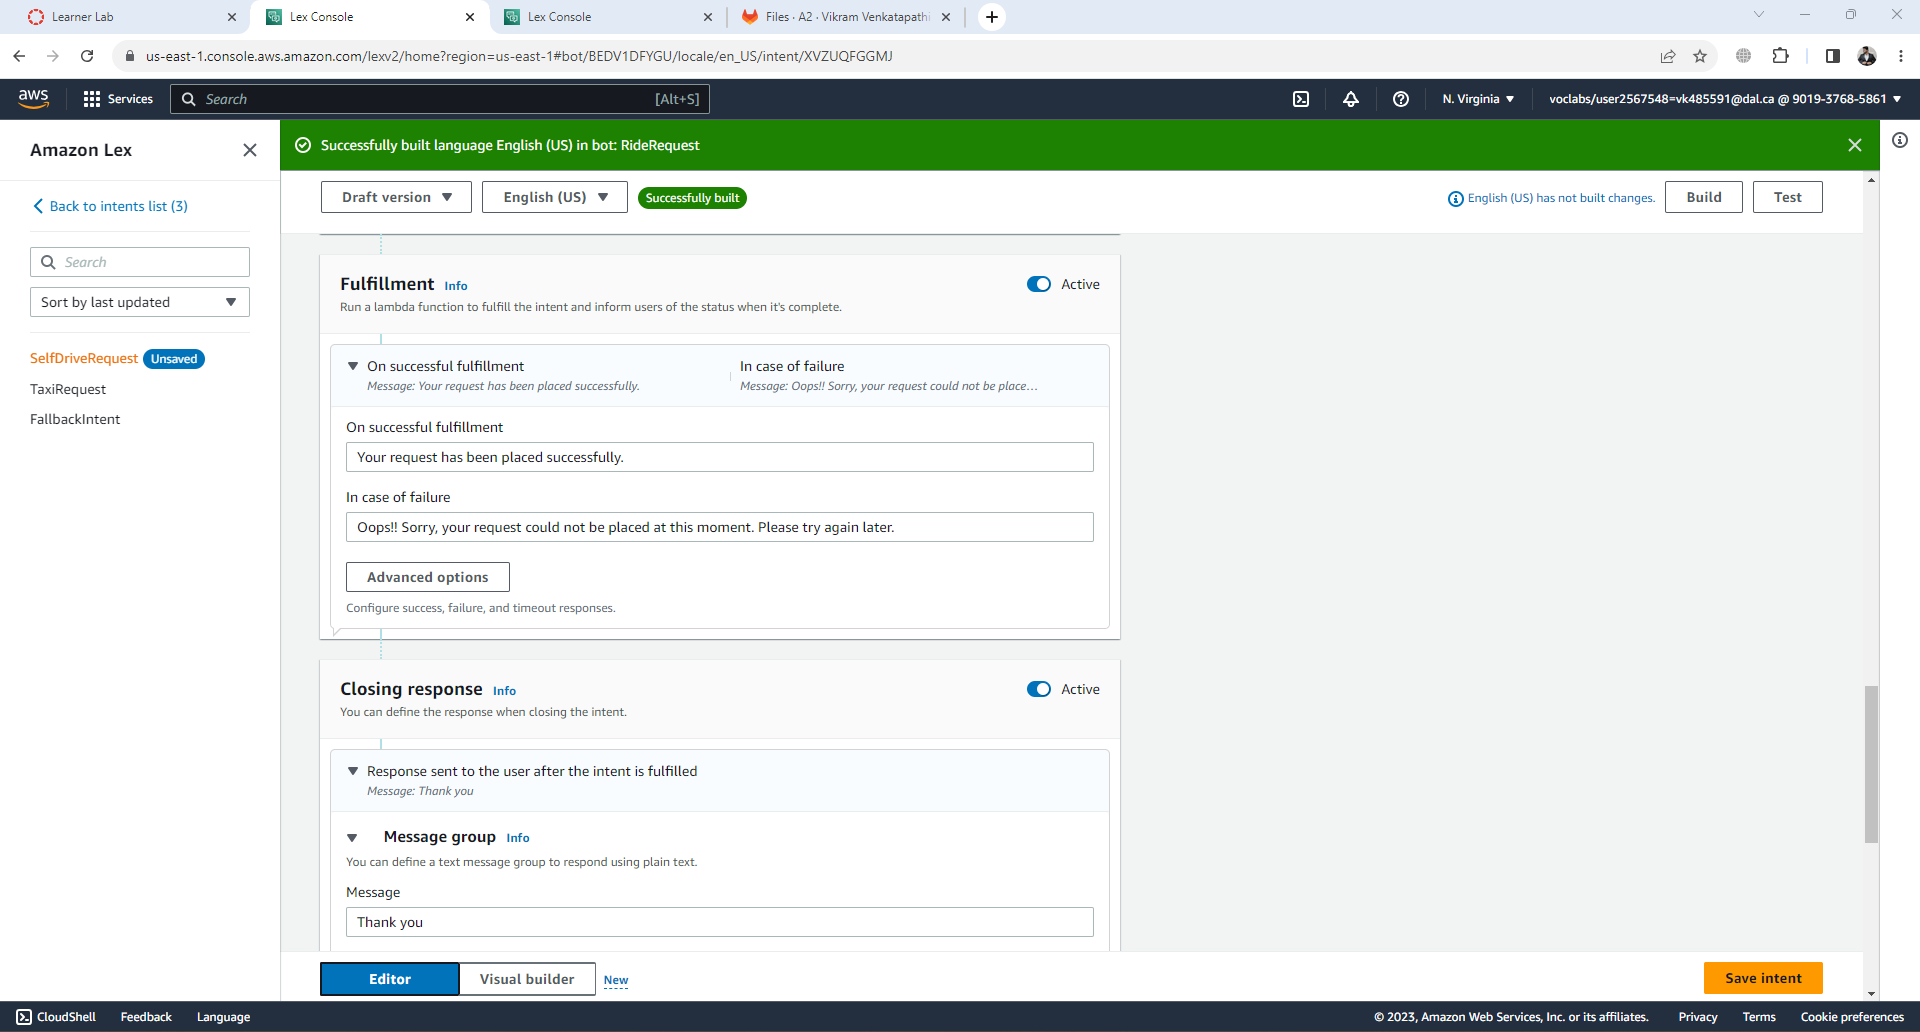
\includegraphics[scale=1, width=15cm,height=7.5cm]{PROBLEM 2/Screenshots/3. Lex/2. Self ride request/3.6 fullfilment prompt and closing response.png}}
    \caption{\textbf{\textit{SelfDriveRequest intent creation - Add Fullfilment prompt and Closing response}}}
    \label{fig:}
\end{figure}

\newpage

\section{Output}
\begin{figure}[htp]
    \centering
    \fbox{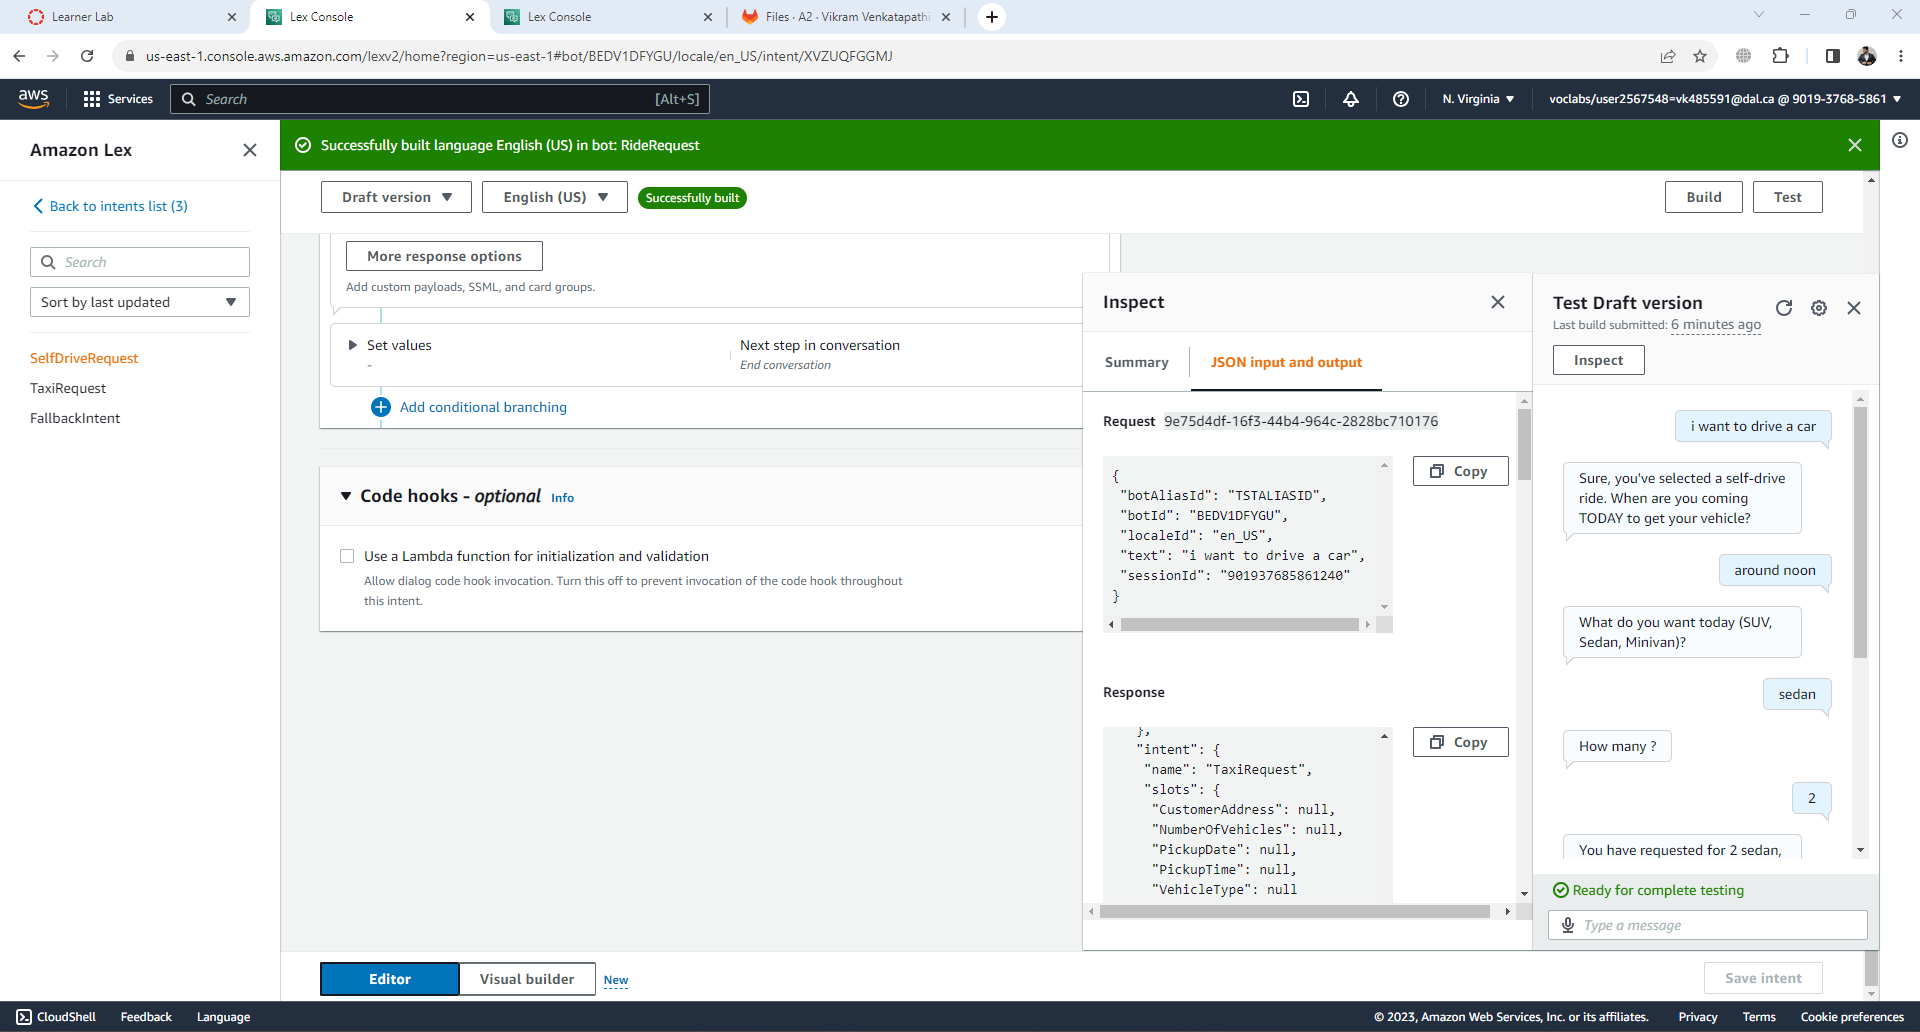
\includegraphics[scale=1, width=15cm,height=7.5cm]{PROBLEM 2/Screenshots/3. Lex/3. Output/1.1 self drive- yes.png}}
    \caption{\textbf{\textit{SelfDrive - Confirm request 1.1}}}
    \label{fig:}
\end{figure}
\begin{figure}[htp]
    \centering
    \fbox{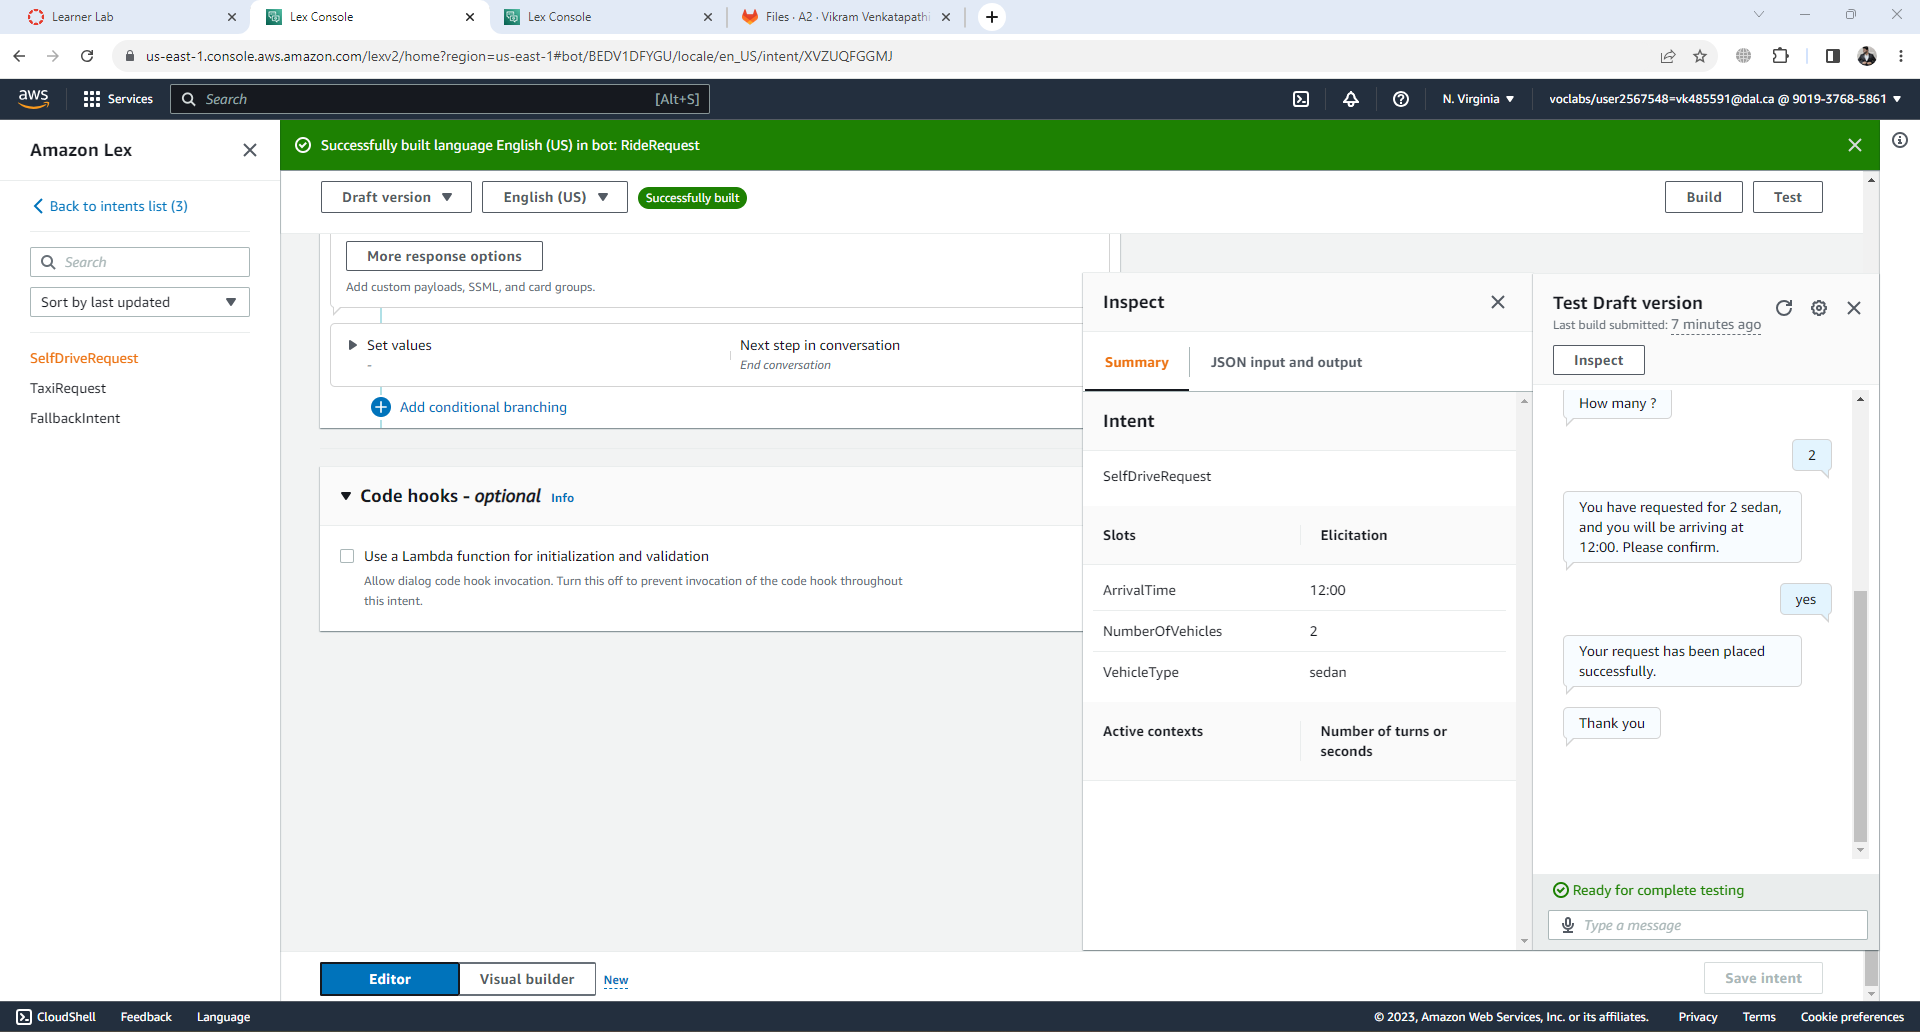
\includegraphics[scale=1, width=15cm,height=7.5cm]{PROBLEM 2/Screenshots/3. Lex/3. Output/1.2 self drive- yes.png}}
    \caption{\textbf{\textit{SelfDrive - Confirm request 1.2}}}
    \label{fig:}
\end{figure}

\begin{figure}[htp]
    \centering
    \fbox{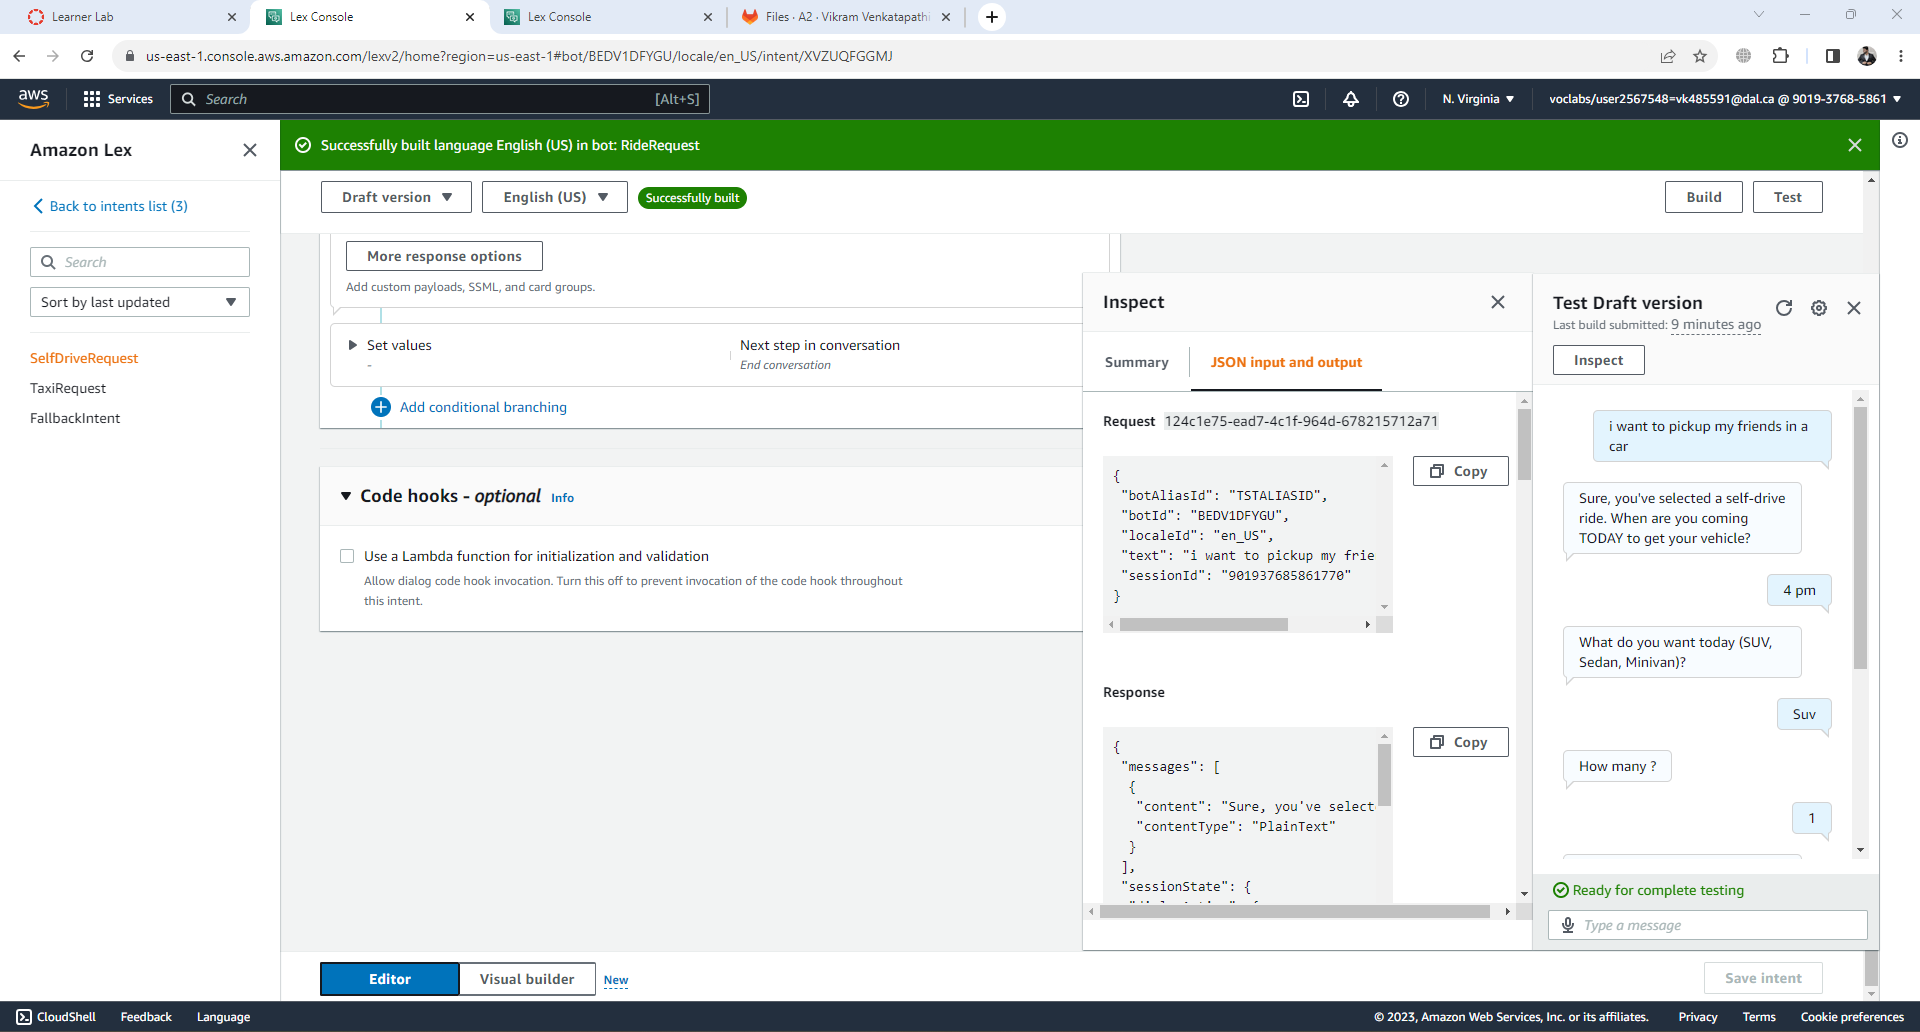
\includegraphics[scale=1, width=15cm,height=7.5cm]{PROBLEM 2/Screenshots/3. Lex/3. Output/2.1 self drive- no.png}}
    \caption{\textbf{\textit{SelfDrive - Cancel request 1.1}}}
    \label{fig:}
\end{figure}
\begin{figure}[htp]
    \centering
    \fbox{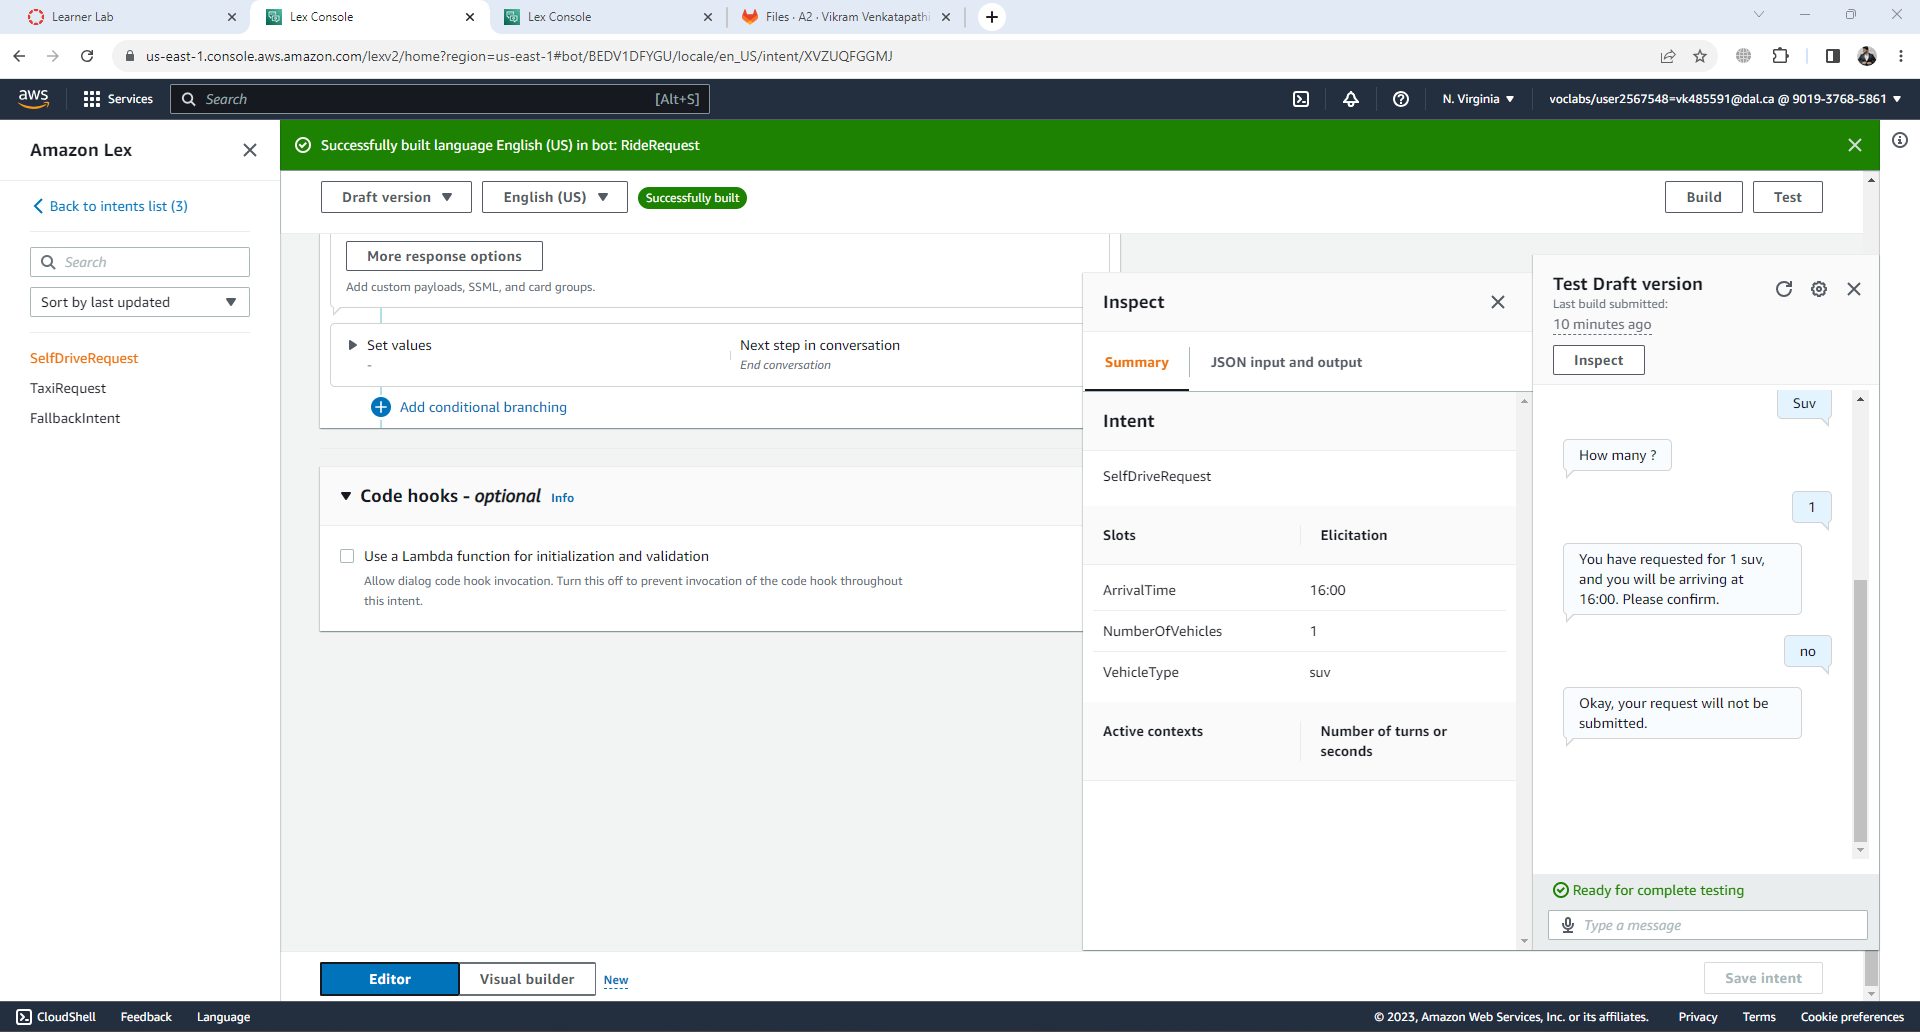
\includegraphics[scale=1, width=15cm,height=7.5cm]{PROBLEM 2/Screenshots/3. Lex/3. Output/2.2 self drive- no.png}}
    \caption{\textbf{\textit{SelfDrive - Cancel request 1.2}}}
    \label{fig:}
\end{figure}

\begin{figure}[htp]
    \centering
    \fbox{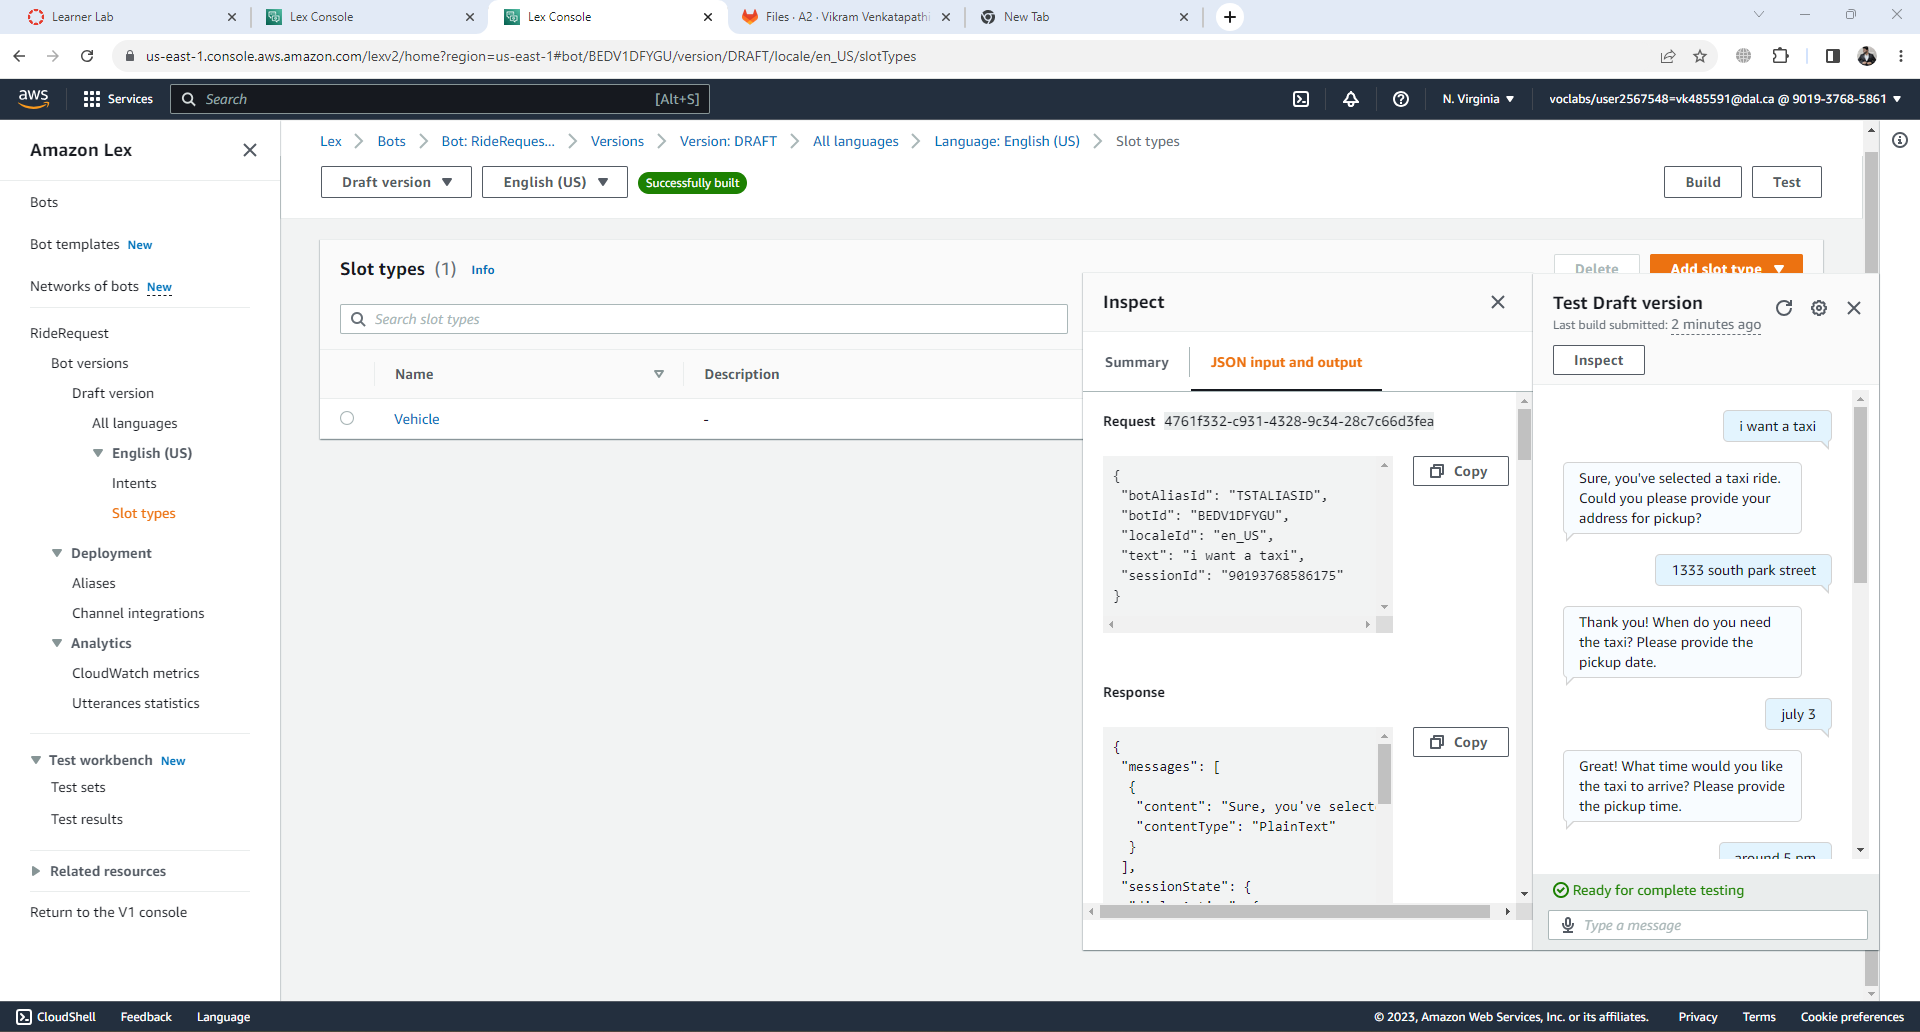
\includegraphics[scale=1, width=15cm,height=7.5cm]{PROBLEM 2/Screenshots/3. Lex/3. Output/3.1 taxi - yes.png}}
    \caption{\textbf{\textit{Taxi - Confirm request 1.1}}}
    \label{fig:}
\end{figure}
\begin{figure}[htp]
    \centering
    \fbox{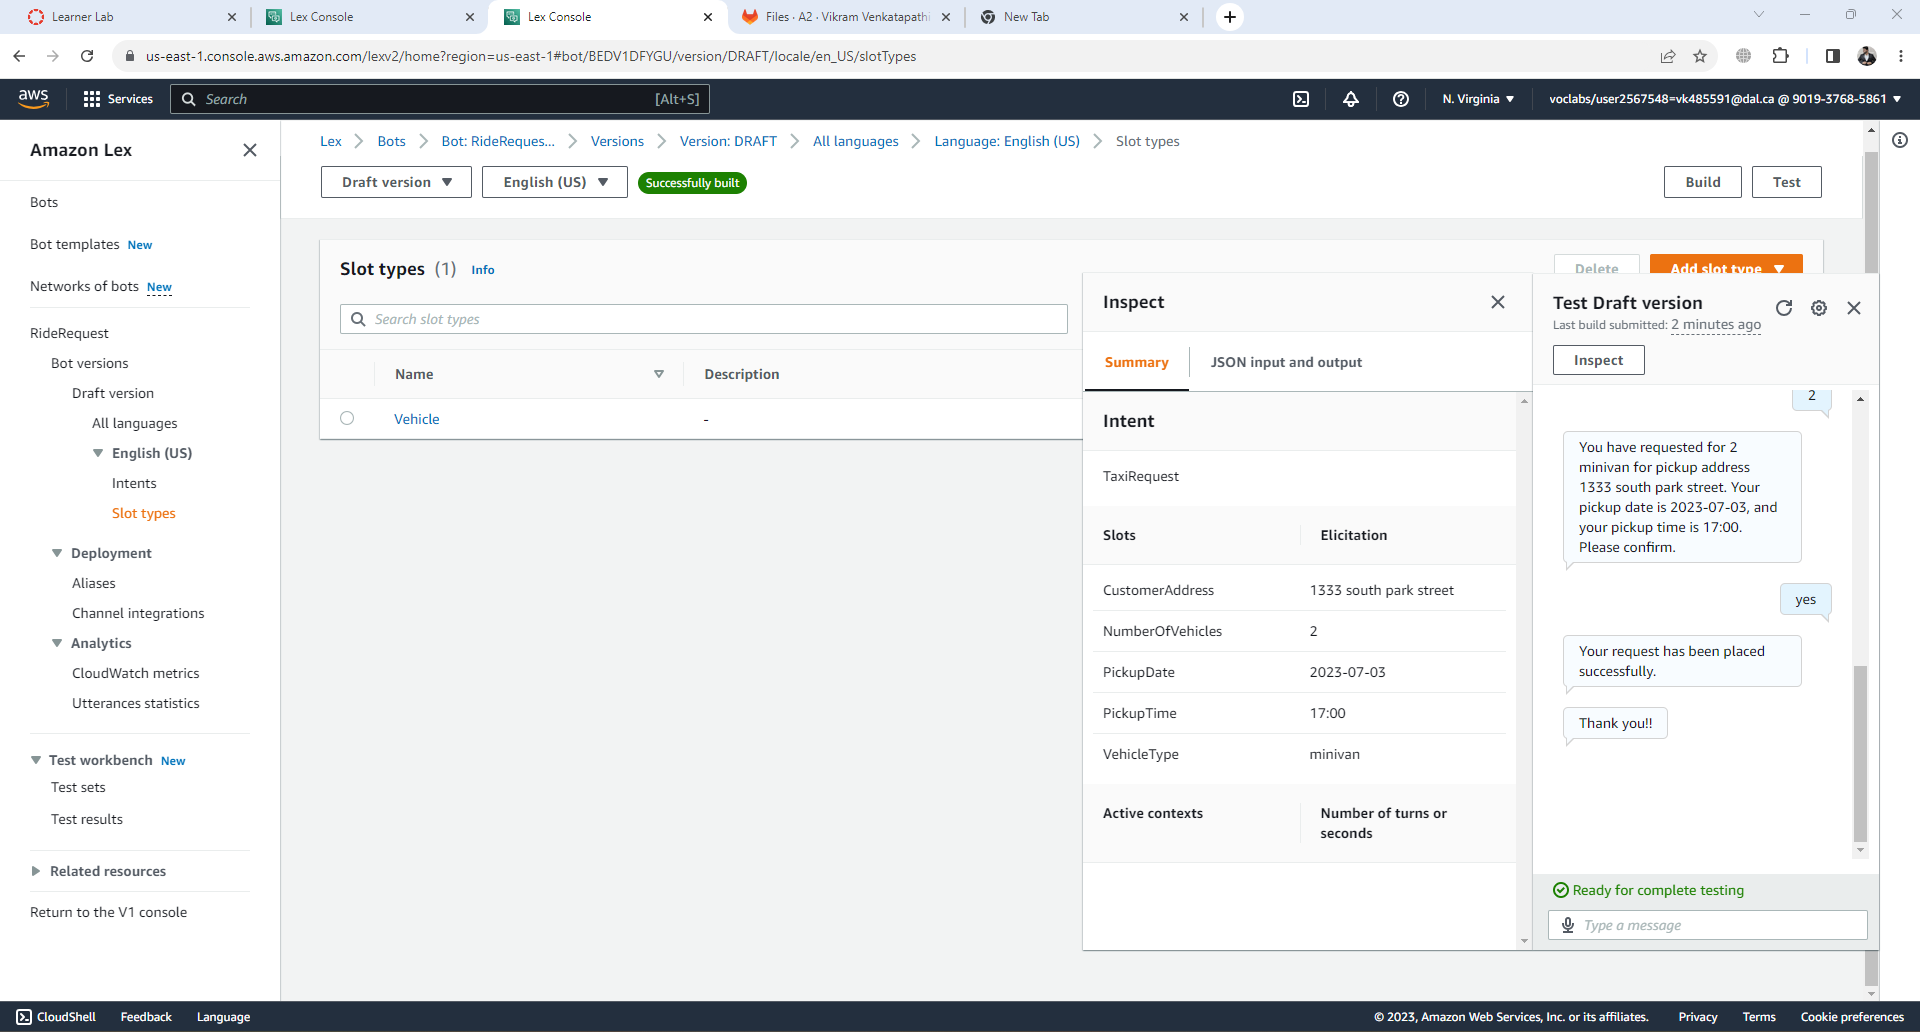
\includegraphics[scale=1, width=15cm,height=7.5cm]{PROBLEM 2/Screenshots/3. Lex/3. Output/3.2 taxi - yes.png}}
    \caption{\textbf{\textit{Taxi - Confirm request 1.2}}}
    \label{fig:}
\end{figure}

\begin{figure}[htp]
    \centering
    \fbox{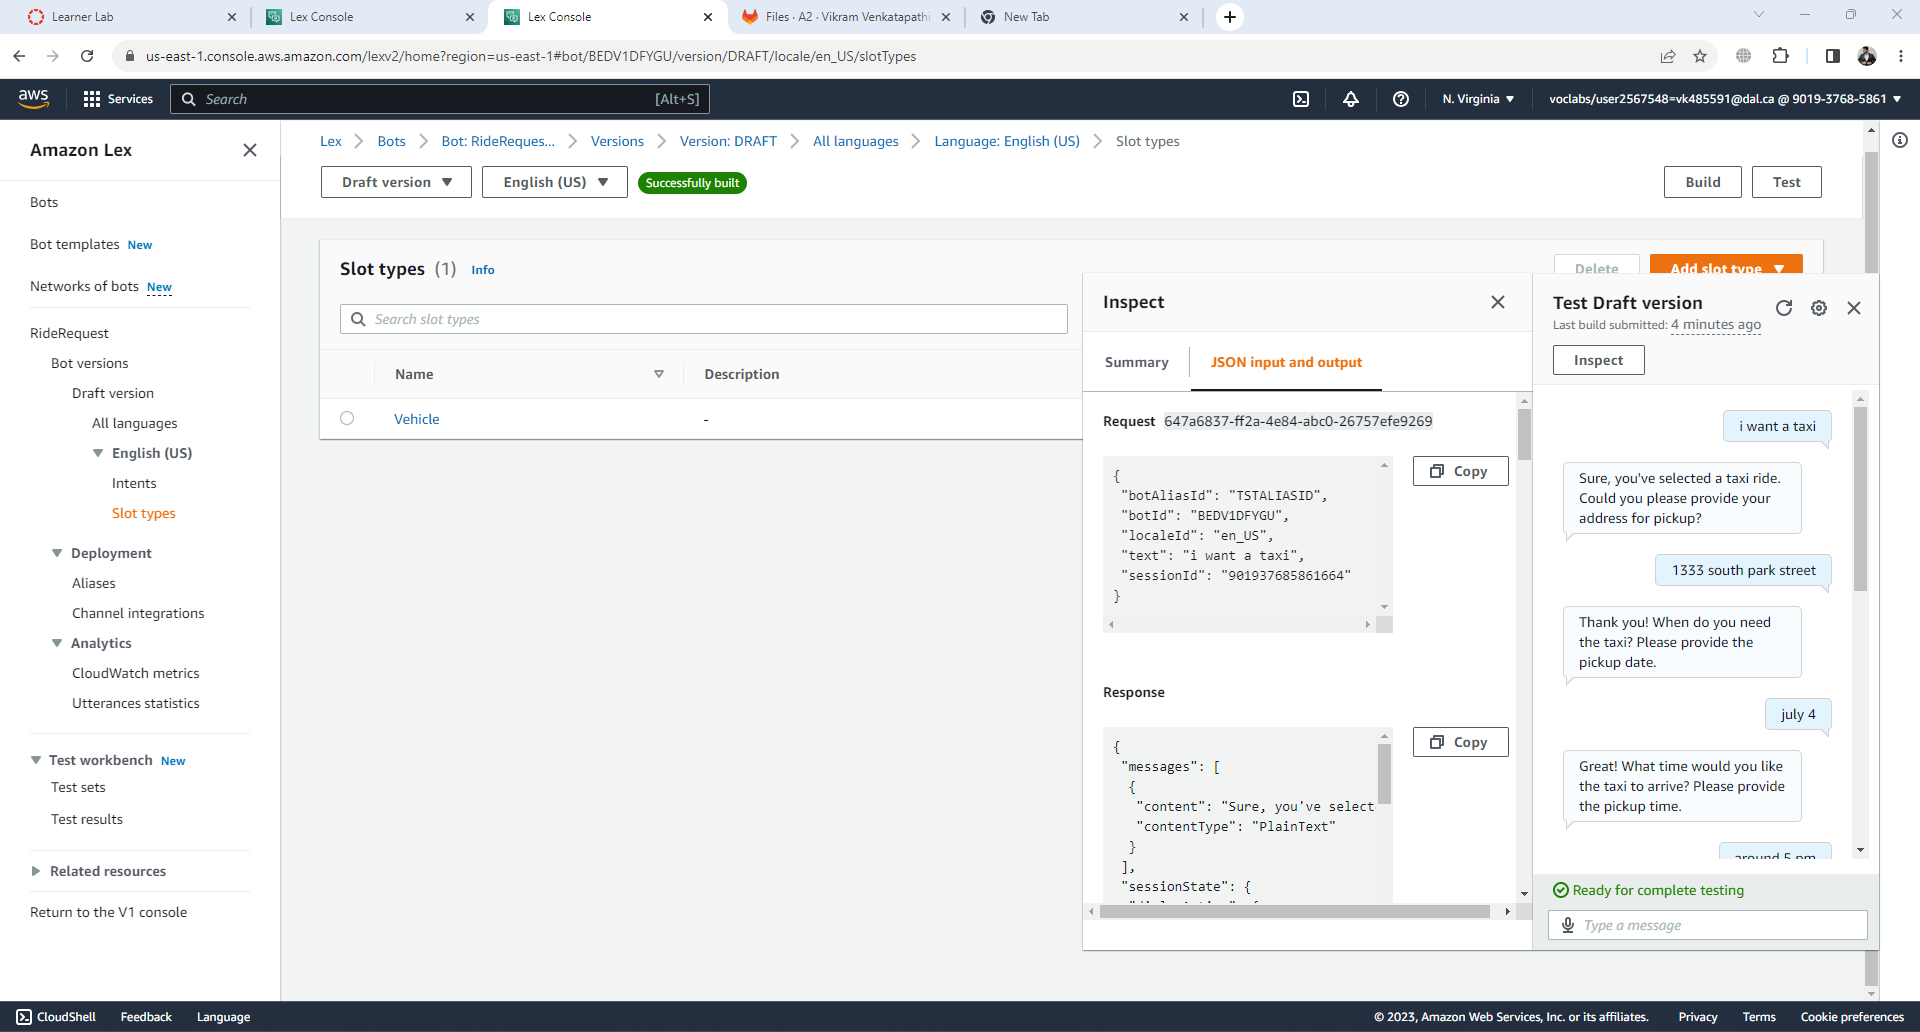
\includegraphics[scale=1, width=15cm,height=7.5cm]{PROBLEM 2/Screenshots/3. Lex/3. Output/4.1 taxi - no.png}}
    \caption{\textbf{\textit{Taxi - Cancel request 1.1}}}
    \label{fig:}
\end{figure}
\begin{figure}[htp]
    \centering
    \fbox{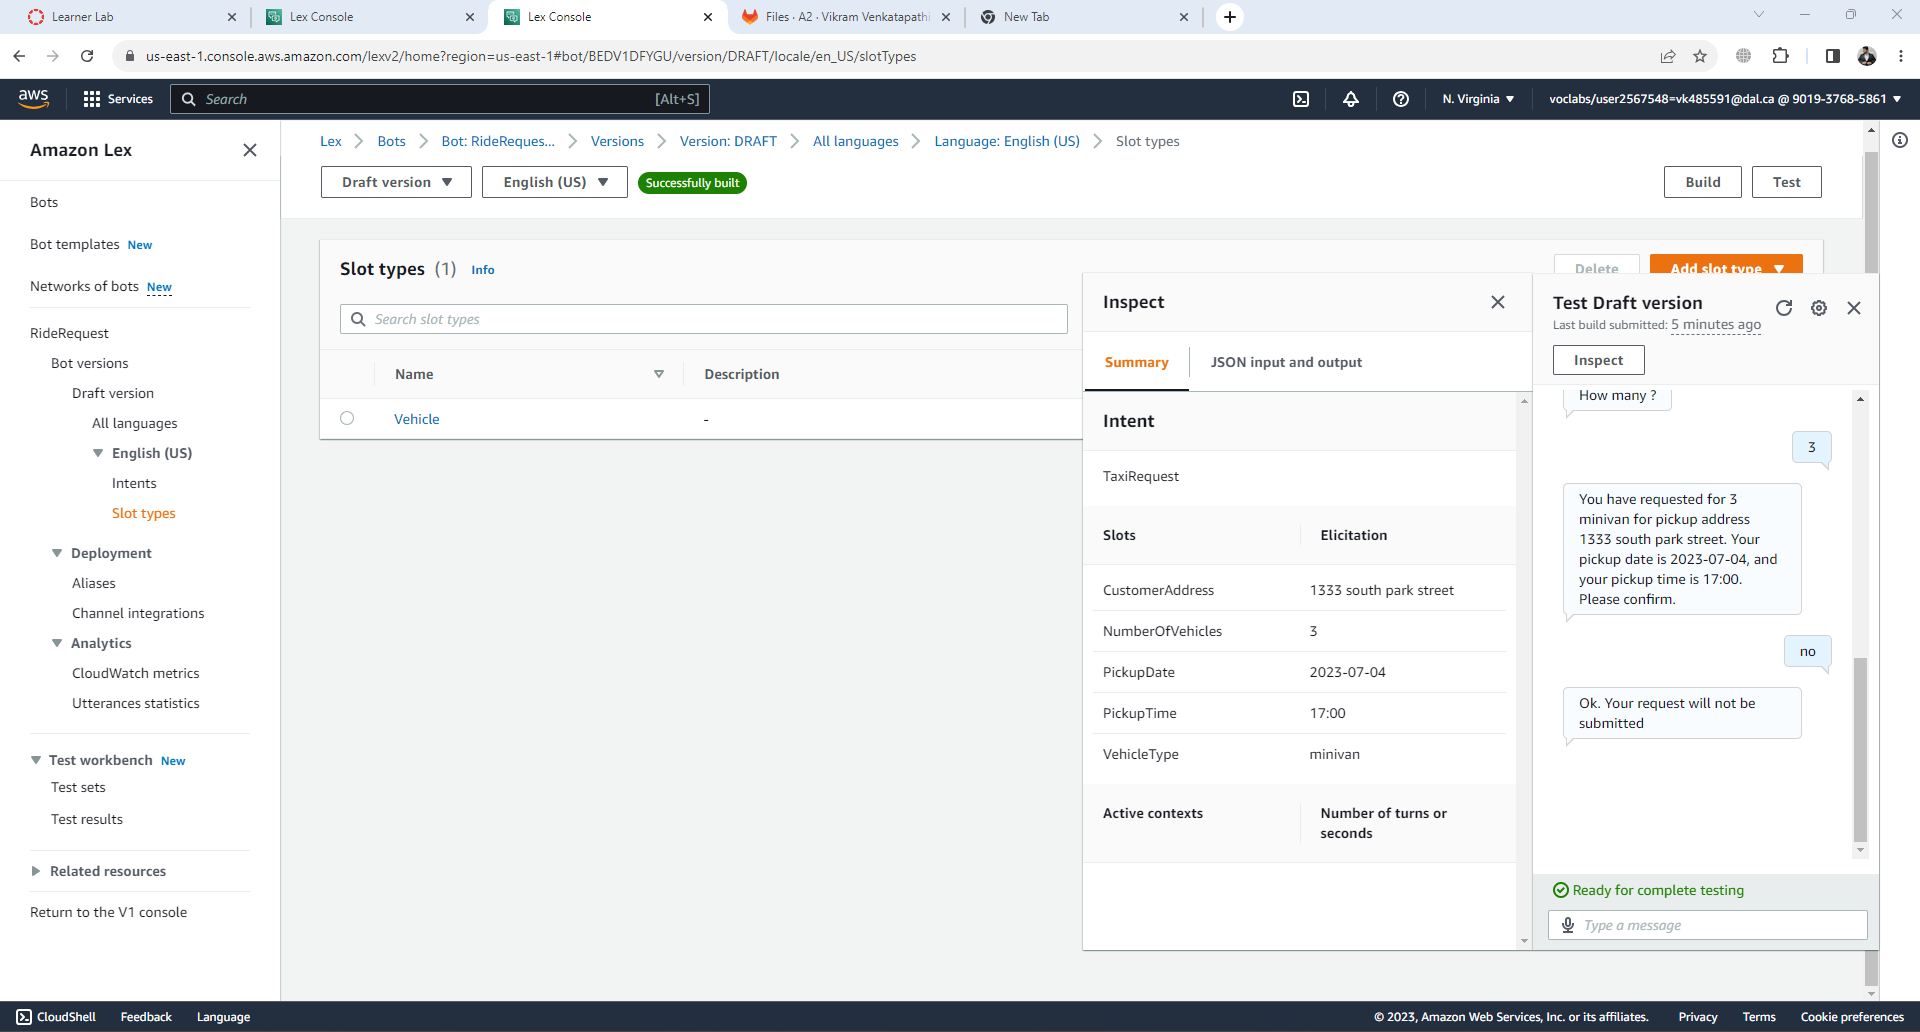
\includegraphics[scale=1, width=15cm,height=7.5cm]{PROBLEM 2/Screenshots/3. Lex/3. Output/4.2 taxi - no.png}}
    \caption{\textbf{\textit{Taxi - Cancel request 1.2}}}
    \label{fig:}
\end{figure}


% \begin{figure}[htp]
%     \centering
%     \fbox{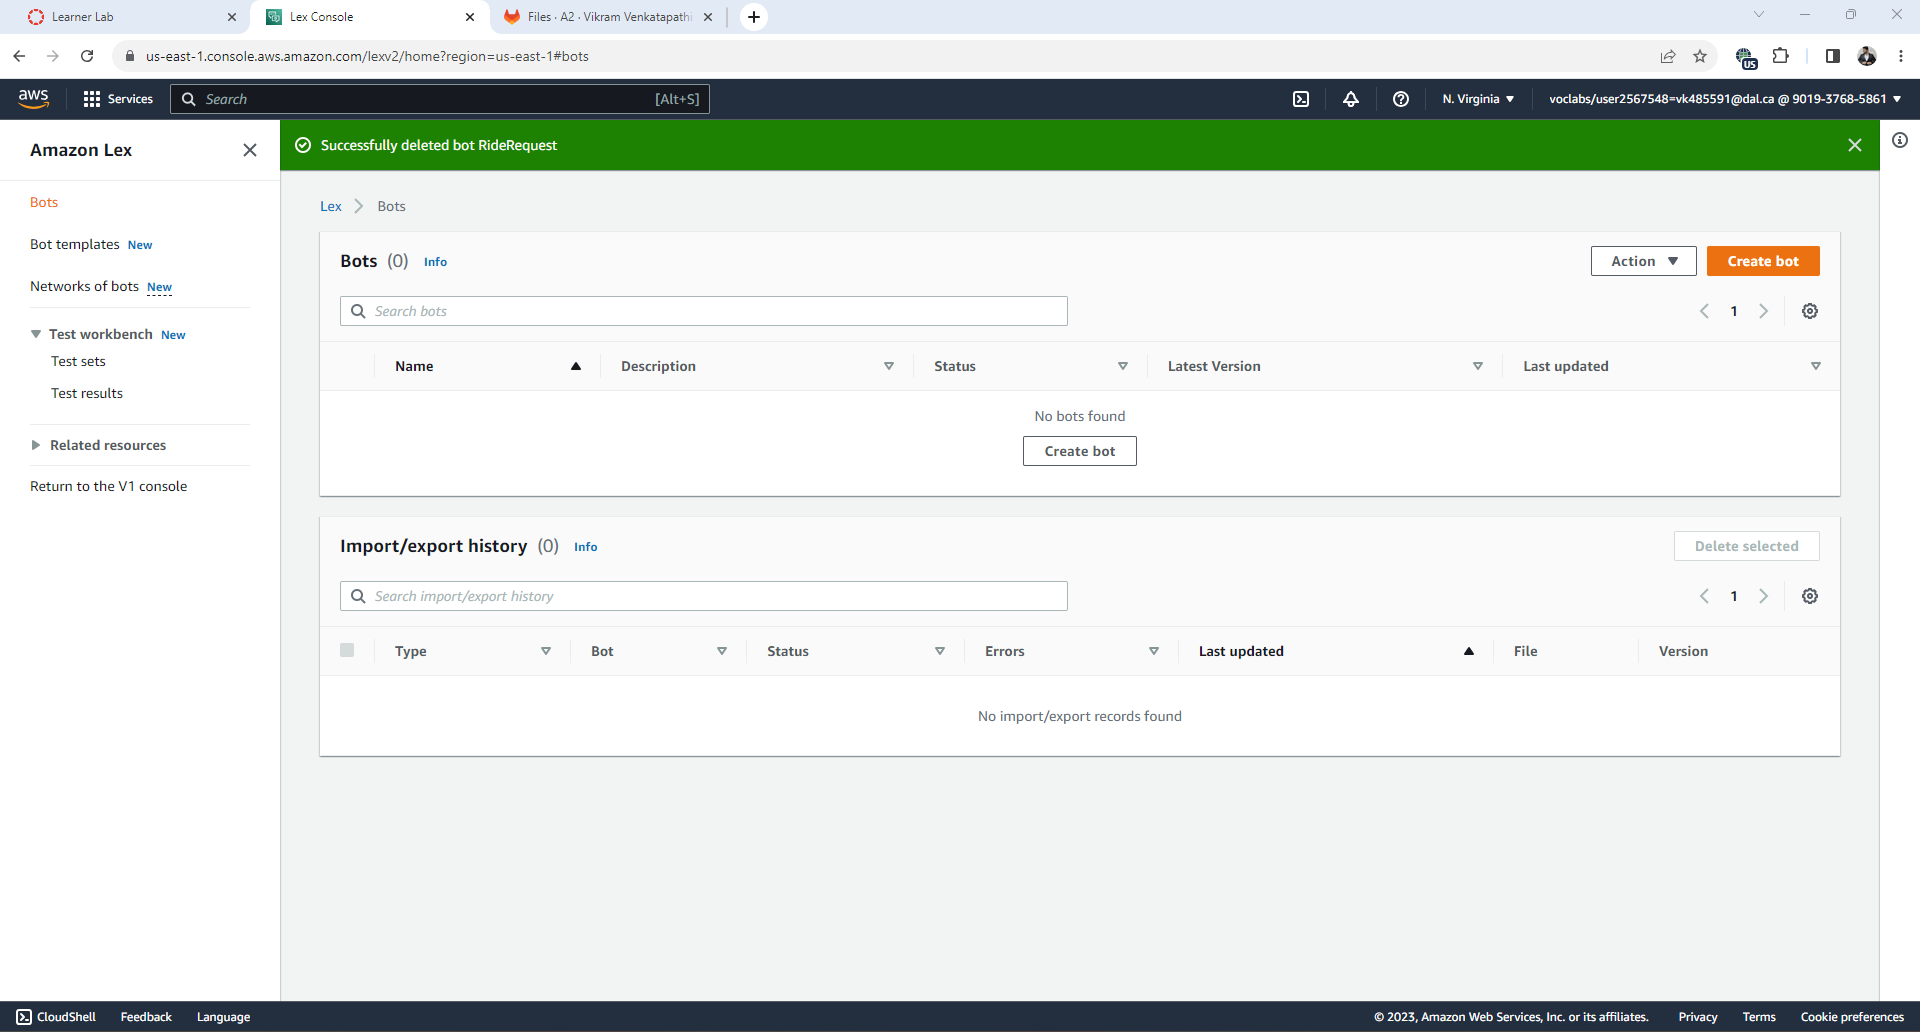
\includegraphics[scale=1, width=15cm,height=7.5cm]{PROBLEM 2/Screenshots/3. Lex/0. Empty bots.png}}
%     \caption{\textbf{\textit{}}}
%     \label{fig:}
% \end{figure}